\documentclass[12pt]{article}
%\usepackage{lgrind}

\usepackage[square,comma,numbers,sort&compress]{natbib}
\usepackage{amsmath,amsthm,amssymb,amsfonts,amsbsy,latexsym}
\usepackage{graphics}
\usepackage{epsfig}
%\usepackage[hang,raggedright]{subfigure}
\usepackage{epsf}
\usepackage{setspace}
\usepackage{hangcaption}
\usepackage{graphicx}    % needed for including graphics e.g. EPS, PS
\usepackage{multirow}
\usepackage{threeparttable}
\usepackage{cancel}
\usepackage{enumerate}
\usepackage{color}
\usepackage{hyperref}

\usepackage{algorithmicx}
\usepackage[ruled]{algorithm}
\usepackage{algpseudocode}
\usepackage{varwidth}
\usepackage{caption}
\usepackage[font=small]{subcaption}
\usepackage{longtable}
\usepackage{mathrsfs}

\hypersetup{
    colorlinks=true,       % false: boxed links; true: colored links
    linkcolor=black,          % color of internal links
    citecolor=black,        % color of links to bibliography
    filecolor=magenta,      % color of file links
    urlcolor=blue           % color of external links
}

\newcommand{\R}{{\mathbb{R}}}
\newcommand{\bit}{\begin{itemize}}
\newcommand{\eit}{\end{itemize}}
\newcommand{\red}[1]{{\color{red}{#1}}}

\graphicspath{{./figures/}}

\begin{document}
\raggedbottom %avoid weird vertical justification

\title{Model Adaptivity for Goal Oriented Inference using Adjoints}

 \author{}%Vikram V. Garg, Roy H. Stogner
% \affil{vikram@ices.utexas.edu, roystgnr@ices.utexas.edu}
% \affil{Institute for Computational and Engineering Sciences, University of Texas, Austin, Texas 78712}
 \date{}
\maketitle

\begin{abstract}
Inference problems are often constrained by state equations, which arise from conservation laws, and constitutive relations. Often, a hierarchy of models can be derived from such laws and relations, reflecting varying fidelity versus cost tradeoffs. We introduce a goal oriented, model adaptive, inference algorithm, which allows users to achieve an arbitrary error tolerance, while minimizing the use of high fidelity constraints. Numerical experiments exercise the algorithm on a highly nonlinear inverse problem, and showcase the computational savings and robustness benefits of this new approach.

\end{abstract}

\section{Introduction}

Parameter estimation/inference is an important component of mathematical modeling. The ability to infer parameters via an inverse problem allows practitioners to gain important information about systems, processes and the models that are used to describe them. Such inference also avoids intrusive experiments, which may otherwise be prohibitively expensive or excessively intrusive. Once parameters have been inferred via an inverse problem, they can be used for forward propogation of the model and computing relevant goals and quantities of interest for the modeling/decision making process.

Data, constraints and prior information form the critical components of an inverse problem formulation. There is an extensive literature pertaining to all these components, pertaining to the ascription/filtering of noise in data, the choice of regularization/prior information, the efficient incorporation of constraints in solving the problem and so on. Specifically, the work on the constraints or 'state equations' in the inverse problem focuses on methods to reduce the computational expense of solving/inverting the models that represent them. Such work includes the use of reduced order models to represent constraints, adaptive mesh refinement to control the size of the state equations among other strategies.

Models that represent phenomena and processes can usually be organized in a hierarchy according to their fidelity and expense. The use of multiple models simultaneously for forward simulation is well established. In this work, we extend the use of the multi-fidelity models to inverse problems. We present a systematic method to use different constraints in different regions of the domain, while controlling the error due to the use of lower fidelity models in a target quantity of interest. Our approach is based on a novel use of adjoint error estimation, which enables the computation of third-order QoI error estimates, at the cost of solving an additional adjoint problem. 

The rest of the paper is organized as follows, Section~\ref{} presents the mathematical formulation and error analysis for the multi-model inverse problem. Then, in Section~\ref{} we discuss the goal oriented inference algorithm and its application to a model problem and a contaminant flow problem. Finally, we present conclusions and direction for future work in Section~\ref{}.

\subsection{draft outline}
\bit 
\item background/previous work? to put this work in context?
  %this is probably enough? at least for previous work...
  %what context though? is this another way to approach inverse problems?
\item mathematical formulation
  \bit
  \item define inverse problem and qoi
  \item derive error estimate
  \item caveats (models to which this can be applied, no guarantee that mixed model will be worth the cost to obtain, no bounds on accuracy of estimate in nonlinear case)
  \item relation to mesh refinement
  \item How does this compare to just using Oden et al's method (multimodel, foward with QoI) and replacing forward PDEs with optimality system of inverse problem? (Oden's gets you second-order in error psiHF-psiLF, but this one gets third, though you have to compute the super-adjoint...linear solve, though...big system, but linear...)
    %solving for adjoint and forward simultaneously (KKT) might cause you to lose an order of accuracy?
    %where was that book that Oden might have mentioned inverse application of his method?
      %Multiscale methods : bridging the scales in science and engineering / edited by Jacob Fish. (TA335.M85 2010 in barker)
  \eit
\item numerical results (perhaps not include all of these...)
  \bit
  \item convection-diffusion(-reaction)
    \bit
    \item interpretation of error estimate breakdown (interaction of QoI with observations)
    \item large reaction term: MF model more cooperative with nonlinear solver
    \eit
  \item convection-diffusion-reaction, field vs scalar description of parameters
    \bit
    \item interface question: do we enforce continuity between the two models' parameters?
      %-navierstokes+stokes seems to require continuity of flux and velocity across boundary...?
      %-is it okay to mix diff and convdiff for the forward like we did? does the discontinuous velocity break any intergration-by-parts   assumptions? (no that's only if discontinuity in diffusion bit...)
    \item chose to have one 'scalar' parameter, so all sections where the LF used shared same single parameter; is this necessarily the best choice?
    %alternative way to describe 'scalar' case? but here we say there is one scalar, so this would be how to combine them...if you wanted plateaus to be different, can let LF model be two-scalars...
    %fig 3.10 -> what does the inferred field look like? does it look like two different plateaus?
      % practice/T_channel/diff_param_res/with_reaction/long_channel_stash/qoi3_setup02_r4p2_deref/ (pushed 10/3/15)
        %at the very last refinement, most of refined region seems to be two large humps...and a section that looks pretty much like the surrounding scalar...so maybe 3 patches...
    \item chose to enforce continuity (easier to implement; field representation required to be continuous); algorithm wanted 60/40 HF/LF mix
    \eit
  \item alternate/additional example: use setup from B+V? navier-stokes and another model? 
    \bit
    \item potential flow? model flow as sum of elementary flows; but then parameters would be magnitudes of elementary flows, which has no spatial location...is that a problem for the algorithm or just for interpreting error breakdown?
    \item there would still be the question of how to interface the models...(in stokes vs navier-stokes foward paper, they just required continuity of state variables (velocity field and presssure))
    %do scalar + field for infer BCs on BV NS thing? try for different QoIs? (can we have a variable live on a boundary while the rest are inside? vikram will poke roy about implementing)
    %stokes is good in slow flows...not in boundary layer cuz gradient is high...
    %what situation would it make sense to use the LF model in some place?
    \eit
  \item have a separate section to address questions of how to mix models? (interfaces, whether 'scalar' parameter should be the same everywhere)
  \eit
\item conclusion...what goes in this section usually? summary and directions for future work?
\eit

\section{Mathematical Formulation}\label{sect:form}
%
We first introduce the goal oriented inverse problem formally, providing definitions and optimization, variational statments. Then we will derive a rigorous, a posteriori error estimate for the error induced in the QoI due to the use of mixed/lower fidelity constraints.

%------------------------------------------------------------------------------%
\subsection{Problem Setup}  \label{sec:setup}
%------------------------------------------------------------------------------%
%
We seek to infer an unknown parameter $q \in Q$, where $Q$ is a Hilbert space. Consider a state variable $u \in U$, which satisfies a bilinear form $a:U \times U \to \Reals$, such that,
%
\begin{equation}
\label{eq:weakForm}
a(u,q)(\phi)=\ell(q)(\phi),\quad\forall\phi\in U,
\end{equation}
%
where the form $a$ and functional $\ell$ are linear with respect to the arguments in the second pair of parentheses. Further, we define an observation operator $C:U\to\Reals^{n_d}$ that maps the state to $n_d$ predicted observations. The actual observations (data) are denoted by $d\in\R^{n_d}$. 

The unknown parameter $q$ can then be inferred by minimizing the difference between the predicted and actual observations, leading to an inverse problem. Such inverse problems are typically ill-posed, since the observations are sparse, and insufficiently informative to uniquely determine the parameters. To make the inverse problem well-posed, a regularization, denoted by $R(q)$, is used to inject prior information or beliefs about the parameters into the formulation. The regularized inverse problem can thus be written as a constrained optimization problem,
%
\begin{subequations}
\label{eq:invOpt}
\begin{align}
\min\limits_{q,u} & \quad J(q,u)=\frac{1}{2}\|d-C(u)\|_2^2 + R(q) \label{eq:invOpt_obj} \\
\textrm{s.t. }& \quad a(u,q)(\phi)=\ell(q)(\phi),\quad\forall\phi\in U \label{eq:invOpt_cons}
\end{align}
\end{subequations}
%
where we aim to minimize the cost function $J$, which includes the mismatch between predicted and actual observations and a regularization term $R(q)$, subject to the state $u$ and parameters $q$ satisfying the constraints given by Equation (\ref{eq:weakForm}). 

The constraints given by Eq.~\eqref{eq:weakForm} are typically models of physical processes or systems. However, a given physical system need not have a unique model that can describe it; there may be various models of different fidelities. This naturally introduces a hierarchy of models, introducing a tradeoff between fidelity and computational expense. Consider two models with which we infer parameters: the high-fidelity (HF) model and a low fidelity (LF) model. We then have a specific form of Equation (\ref{eq:weakForm}) for the high-fidelity model:
\begin{equation}
a_{HF}(u_{HF},q_{HF})(\phi_{HF})=\ell_{HF}(q_{HF})(\phi_{HF}),\quad\forall\phi_{HF}\in U_{HF},
\end{equation}
where $u_{HF}\in U_{HF}$ and $q_{HF}\in Q_{HF}$. Similarly, the inverse problem in Equation (\ref{eq:invOpt}) has the specific form
\begin{equation}
\begin{array}{r@{}c}
\min\limits_{q_{HF},u_{HF}} & \quad J_{HF}(q_{HF},u_{HF})=\frac{1}{2}\|d-C_{HF}(u_{HF})\|_2^2 + R_{HF}(q_{HF}) \\ \textrm{s.t. }& \quad a_{HF}(u_{HF},q_{HF})(\phi_{HF})=\ell_{HF}(q_{HF})(\phi_{HF}),\quad\forall\phi_{HF}\in U_{HF},
\end{array}
\end{equation}
for which we have the Lagrangian
\begin{equation}
\mathcal{L}_{HF}(q_{HF},u_{HF},z_{HF})= J_{HF}(q_{HF},u_{HF})-(a_{HF}(u_{HF},q_{HF})(z_{HF})-\ell_{HF}(q_{HF})(z_{HF})).
\end{equation}
The lower fidelity model can be similarly defined and identified by the subscript $LF$.

In the case of a goal-oriented inverse problem, the ultimate purpose of inferring the unknown parameters is to calculate some Quantity of Interest (QoI). Assuming a single scalar QoI, we denote this QoI by $I(q,u)$, where $I:Q\times U\to\R$ is a functional that maps the parameters and state to our QoI. Since our ultimate goal is to compute this QoI, the particular tradeoff we consider is the fidelity and resultant computational expense of the model we use, versus the error in the QoI. We thus seek to introduce the QoI functional $I$ into the inverse problem formulation, by introducing auxilary variables and additional adjoint equations. Then we use this formulation to derive an a posteriori error estimate for $I$, where the errors considered are those which occur due to the use of constraints other than those given by Eq.~\eqref{eq:invOpt_cons}.
%
%------------------------------------------------------------------------------%
\subsection[Error Estimate for a Goal-Oriented Inverse Problem]{Error Estimate for a Goal-Oriented Inverse \\Problem}  \label{sec:deriv}
%------------------------------------------------------------------------------%
%
For a given hierarchy of models, consider the QoI calculated from inferring the parameters with the highest-fidelity model; we take this QoI to be the value with which we compare other QoI estimates. In this section we derive an a posteriori estimate for the error in the QoI from inferring the parameters with a lower-fidelity model, as compared to that which would have resulted from solving the inverse problem with the highest-fidelity model. The main result is,
%
\begin{theorem}
\label{thm:error_estimate}
Following the notation established in section~\ref{sec:setup}, let the bilinear form $a:U \times U \to \Reals$ be three times continuously differentiable with respect to the state $u$ and parameters $q$. Let the observation operator $C:U\to\Reals^{n_d}$ be three times continuously differentiable with respect to the state $u$. Also, let the regularization operator $R:Q\to\Reals$ be differentiable with respect to the parameter $q$, and the functional $I:Q\times U\to\Reals$ be differentiable with respect to the state $u$ and parameter $q$.

Consider the Lagrangian equation induced by Eq.~\eqref{eq:invOpt},
%
\begin{equation}
\label{eq:InvsOpt_lag}
\mathcal{L}(q,u,z)= J(q,u)-(a(u,q)(z)-\ell(q)(z)),
\end{equation}
%
where $z\in U$ is the adjoint. Denoting the primary variables as $\xi=(q,u,z)$, introduce corresponding auxiliary variables $\chi=(p,v,y)\in Q\times U\times U$. Let the augmented Lagrangian be defined as,
%
\begin{equation}
\label{eq:InvsOpt_auglag}
\mathcal{M}((q,u,z),(p,v,y)) = I(q,u) + \mathcal{L}_{quz}'(q,u,z)(p,v,y),
\end{equation}
%
where $\mathcal{L}_{quz}'(q,u,z)(p,v,y)$ denotes the Fr\'{e}chet derivative of the Lagrangian about the primary variables $(q,u,z)$, in the direction of the auxiliary variables $(p,v,y)$. Let $\Psi = (\xi_\Psi,\chi_\Psi)$ denote the stationary point of $\mathcal{M}$.

Denote by $\Psi_{HF}$ and $\Psi_{LF}$, stationary points of the high and low fidelity versions of Eq.~\eqref{eq:InvsOpt_auglag} and, consider the adjoint problem,
%
\begin{equation}
\label{eq:superAdjEq}
\mathcal{M}'_{HF,\Psi}(\Lambda;\Psi_{HF})(\Phi)=\mathcal{Q}(\Phi)=\mathcal M'_{HF}(\Psi_{LF})(\Phi),\quad\forall\Phi\in(Q_{HF}\times U_{HF}\times U_{HF})^2,
\end{equation}
%
for the supplementary adjoint $\Lambda$. Then, the error in the Quantity of Interest $I$ is given by,
%
\begin{multline}
\label{eq:finErrExp}
I(q_{HF},u_{HF})-I(q_{LF},u_{LF})=\\-\frac{1}{2}\mathcal{M}'_{HF,\Psi}(\Psi_{LF})(\Lambda)+\mathcal M_{HF}(\Psi_{LF})-\mathcal M_{LF}(\Psi_{LF})+\mathcal{R}(e^3).
\end{multline}
%
\end{theorem}
%
\begin{proof}
%
Observe that,
%
\begin{equation}
\label{eq:MeqI}
\mathcal{M}(\Psi)=I(q,u),
\end{equation} 
%
since taking variations of $\mathcal{M}$ with respect to the auxiliary variables gives that $\xi_\Psi$ is a stationary point of $\mathcal{L}$.

Extending the property in Equation (\ref{eq:MeqI}) to the augmented Lagrangians for the high and low fidelity models, we have,
%
\begin{multline}
\label{eq:repIwithM}
I(q_{HF},u_{HF})-I(q_{LF},u_{LF})=\\\mathcal{M}_{HF}(\Psi_{HF})-\mathcal{M}_{HF}(\Psi_{LF})+\mathcal{M}_{HF}(\Psi_{LF})-\mathcal{M}_{LF}(\Psi_{LF})\textrm{.}
\end{multline}
%
Applying Proposition 3 from~\cite{BecVex05} for the difference $\mathcal{M}_{HF}(\Psi_{HF})-\mathcal{M}_{HF}(\Psi_{LF})$,  
\begin{equation}
\mathcal{M}_{HF}(\Psi_{HF})-\mathcal{M}_{HF}(\Psi_{LF}) = \frac{1}{2}\mathcal{M}'_{HF,\Psi}(\Psi_{LF})(\Psi_{HF}-\Psi_{LF})+\mathcal{R}(e^3)\textrm{,}
\end{equation}
where $\mathcal{R}$ is a remainder term that is third-order in the error $e=\Psi_{HF}-\Psi_{LF}$. Combining Equations (\ref{eq:repIwithM}) and (\ref{eq:preadj}) we obtain
\begin{multline}
\label{eq:preadj}
I(q_{HF},u_{HF})-I(q_{LF},u_{LF})=\\\frac{1}{2}\mathcal{M}'_{HF,\Psi}(\Psi_{LF})(\Psi_{HF}-\Psi_{LF})+\mathcal{M}_{HF}(\Psi_{LF})-\mathcal{M}_{LF}(\Psi_{LF})+\mathcal{R}(e^3)\textrm{.}
\end{multline}

Further, the error in the output $\mathcal{Q}$ defined in Equation (\ref{eq:superAdjEq}) can be expressed as a dual-weighted residual,
\begin{equation}
\label{eq:adjOutErr}
\mathcal M'_{HF,\Psi}(\Psi_{LF})(\Psi_{HF}-\Psi_{LF})=-\mathcal{M}'_{HF,\Psi}(\Psi_{LF})(\Lambda).
\end{equation}

Combining Equations (\ref{eq:preadj}) and (\ref{eq:adjOutErr}), we have,
\begin{multline}
I(q_{HF},u_{HF})-I(q_{LF},u_{LF})=\\-\frac{1}{2}\mathcal{M}'_{HF,\Psi}(\Psi_{LF})(\Lambda)+\mathcal M_{HF}(\Psi_{LF})-\mathcal M_{LF}(\Psi_{LF})+\mathcal{R}(e^3).
\end{multline}
%
which completes the proof.
\end{proof}
%
The above error estimate is general and the lower-fidelity model can also be a mixed-fidelity model that combines the high- and low-fidelity model. Given a low-fidelity model and a high-fidelity model, an intermediate, mixed-fidelity (MF) model can be formed by using the high-fidelity model in some parts of the domain, and the low-fidelity model in the rest of the domain.

\section{Numerical Experiments}\label{sect:numexp}
%
We now use Algorithm~\ref{alg:refSeries} to solve goal oriented inverse problems in a multi-model setting. We consider two kinds of multi-fidelity models, in a total of three experiments. In the first experiment, the high fidelity model is a convection-diffusion-reaction nonlinear model, and the low fidelity model is a linear convection-diffusion model. We examine how the localized error estimate is affected by changes in sensor placement and in the QoI region. In the second experiment, the high fidelity model uses an infinite dimensional (field) representation of the inferred parameter, while the low fidelity model uses a scalar representation. \red{The third experiment has the same setting as the first one, except a highly nonlinear version of the reaction term is considered, and showcases the robustness and computatioanal cost benefits of using the adaptive algorithm.}

%In all experiments, starting the simulation with the low fidelity model, we seek to add regions of high fidelity, until the estimated relative error in the target QoI is less than 1$\%$. 

%
\subsection{Error Estimate Localization}
%
Algorithm~\ref{alg:refSeries} does not require a particular method for localizing the error estimate. A na\"{i}ve approach would be to write the error estimate as a sum of integrals over elements and their boundaries, and calculate the error contribution by each element as the integral over that element. While perhaps simple to compute, this method results in non-zero error contributions from elements in which the high-fidelity model is already being used, making the error decomposition more difficult to interpret.

We instead use the alternative method described in \cite{vanOpstaletal15}, decomposing the error estimate into contributions from locally supported basis functions rather than elements. For convenience of notation in this section, we drop subscripts so that $\Psi=\Psi_{LF}$, $Q=Q_{HF}$, and $U=U_{HF}$; for our numerical experiments, we have $Q_{LF}\subset Q$ and $U_{LF}=U$. We note that the error estimate in Equation \ref{eq:finErrExp} can be equivalently written as
%
\begin{equation}
I(q_{HF},u_{HF})-I(q_{LF},u_{LF})=-\frac{1}{2}\mathcal{M}'_{HF,\Psi}(\Psi)(\Lambda)+\mathcal{L}'_{HF,\xi}(\xi_\Psi)(\chi_\Psi)+\mathcal{R}(e^3). \nonumber
\end{equation}
%
We consider a finite-dimensional \red{conforming} subspace $(Q^h\times U^h\times U^h)^3 \subset (Q\times U\times U)^3$ which contains the approximations $(\Lambda^h,\chi_\Psi^h)$. Define a basis $\Phi^h=\{(\varphi,\upvarphi)_i\}_{i\in I}$ consisting of locally supported functions such that span $\Phi^h=(Q^h\times U^h\times U^h)^3$; we can then write $(\Lambda^h,\chi_\Psi^h)=(\sum_{i\in I}\varphi_i\lambda_i,\sum_{i\in I}\upvarphi_i x_i)$. The error estimate
%
\begin{equation}
\epsilon = -\frac{1}{2}\mathcal{M}'_{HF,\Psi}(\Psi)(\Lambda)+\mathcal{L}'_{HF,\xi}(\xi_\Psi)(\chi_\Psi) \leq \sum_{i\in I} \varepsilon_i,
\end{equation}
%
where
%
\begin{equation}\label{eq:basisblame}
\varepsilon_i = \left| -\frac{1}{2}\mathcal{M}'_{HF,\Psi}(\Psi)(\lambda_i\varphi_i)+\mathcal{L}'_{HF,\xi}(\xi_\Psi)(x_i\upvarphi_i) \right|
\end{equation}
%
can be interpreted as the error contribution from the basis function $(\varphi,\upvarphi)_i$. The basis functions with the largest error contributions are flagged, and the elements in their support are refined. Using this method, elements in which the high-fidelity model is already being used are not interpreted as continuing to contribute to the error in the QoI and thus are not marked again for refinement. The only exceptions are elements near the interfaces between the low-fidelity and high-fidelity regions, as basis functions near the boundary may have their support divided between the two regions and thus have a nonzero error contribution. 
%
\subsection{Convection-Diffusion(-Reaction)} \label{sec:cdvcdr}
%
In this section, we consider a pair of models which differ in the physics included. In Section \ref{sec:cdvcdrSetup} we describe a baseline setup for a simple problem in 2D. Section \ref{sec:cdvcdrBaseRef} describes the results of applying Algorithm~\ref{alg:refSeries} to the baseline problem, and Section \ref{sec:qoivdata} describes the results of changing the placement of observations or the QoI region from the baseline.
%
%------------------------------------------------------------%
\subsubsection{Problem Setup} \label{sec:cdvcdrSetup}
%------------------------------------------------------------%
%
We consider a rectangular domain $\Omega(x_1,x_2)=[0,5]\times[0,1]$, where $x_1$ and $x_2$ are the spatial coordinates. The high-fidelity model is a single-species convection-diffusion-reaction equation with a nonlinear reaction term, described by,
%
\begin{subequations}
\label{eq:cdvcdrHF}
\begin{align}
k_d\nabla^2 u - \vec{V}\cdot\nabla u + k_ru^2 = f(q) \quad &\text{in } \Omega, \label{eq:cdvcdrHF_int} \\
u = 0 \quad &\text{on } \partial \Omega \label{eq:cdvcdrHF_bdry}
\end{align} 
\end{subequations}
%
where the state $u$ is the species concentration and $f(q)$ is a forcing field described by the parameters. We have a divergence-free parabolic-profile velocity field $\vec{V}(x_1,x_2) = (2x_2(1-x_2),0)$; the diffusion and reaction coefficients are $k_d = 0.1$ and $k_r = -42.0$, respectively. The low-fidelity model,
%
\begin{equation}
k_d\nabla^2 u - \vec{V}\cdot\nabla u = f(q)
\end{equation}
%
differs only in the removal of the reaction term. To form the mixed-fidelity models, we divide the domain into complementary subdomains, $\Omega_{HF}$ and $\Omega_{LF}$, where the high- and low-fidelity models are solved, respectively. The resulting mixed-fidelity models can be described by, 
%
\begin{equation}
k_d\nabla^2 u - \vec{V}\cdot\nabla u + k^{MF}_ru^2= f(q),
\end{equation}
%
where $k^{MF}_r$ is a piecewise-constant reaction coefficient,
%
\begin{equation}
k^{MF}_r=
\begin{cases}
-42.0 & \textrm{if }x\in\Omega_{HF} \\
0 & \textrm{if }x\in\Omega_{LF}.
\end{cases}
\end{equation}
%
The QoI we wish to calculate is the integral of the state,
%
\begin{equation}
I(q,u)=\int_{(x_1,x_2)\in \Omega_I} u \:\textrm{d}A,
\end{equation}
%
over a region $\Omega_I=[0.625,0.875]\times[0.375,0.625]$. 

The unknown parameters we wish to infer correspond to the forcing field, so that $f(q)=q$. For the low-fidelity model, the inverse problem is linear (the inferred parameters are linear in the observations). Observations consisting of the state at three points in the domain are artificially generated by running the high-fidelity model on a finer mesh with the true forcing field
%
\begin{equation}
f_{true}(x_1,x_2)=
\begin{cases}
1.0 & \textrm{if }(x_1,x_2)\in[0.125,0.375]\times[0.125,0.375] \\
0.8 & \textrm{if }(x_1,x_2)\in[2.375,2.625]\times[0.375,0.625] \\
0 & \textrm{otherwise}.
\end{cases}
\end{equation}
%
The locations of the observations and the region $\Omega_I$ over which the QoI is calculated are shown in Figure~\ref{fig:baseSetup}. Since the inverse problem is ill-posed, we use Tikhonov regularization~\cite{EngHanNeu00}; the regularization term is $\frac{\beta}{2}\int_\Omega \|\nabla f(q)\|_2^2\:\textrm{d}A$, where $\beta=10^{-5}$ is the regularization coefficient. 
%
\begin{figure}[h]
\centering
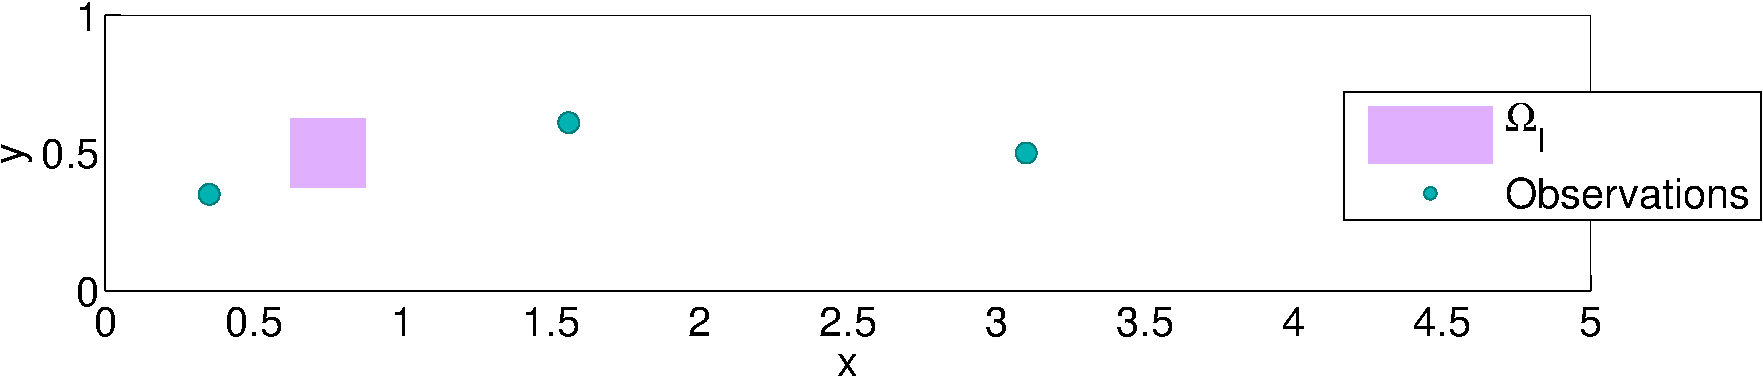
\includegraphics[width=0.8\textwidth]{baseSeries/setup_3_3.pdf}
\caption{Locations of the observations and the QoI region. \red{Aaaah spatial coordinates are not $x$ and $y$! ($y$ is one of the auxiliary variables...)}}
\label{fig:baseSetup}
\end{figure}
%

For the numerical simulations, we use the finite element method (FEM), employing a continuous Galerkin formulation with Lagrange elements. We use the \texttt{libMesh} library~\cite{libMeshPaper} for the FEM calculations. \red{The library offers easy calculation of adjoint systems, error estimates and subdomain restricted variables.}\footnote{But we don't use Libmesh's error estimates or restrict variables to subdomains...} The domain is discretized by a regular mesh of quadrilaterals, with 50 and 250 elements along the short and long boundaries, respectively, for a total of 12,500 elements, resulting in a total of 38,403 degrees of freedom. The diffusion coefficient is chosen so that the cell P\'{e}clet number never exceeds 0.1, and thus no stabilization is required.
%
%------------------------------------------------------------%
\subsubsection{Adaptive Model Refinement Results} \label{sec:cdvcdrBaseRef} 
%------------------------------------------------------------%
%
We now present the results for solving the inference problem using Algorithm~\ref{alg:refSeries}. Once the QoI error estimate is calculated using Equation~(\ref{eq:finErrExp}), the error estimate is then decomposed into local contributions, as described in Equation~(\ref{eq:basisblame}). At each iteration, based on this decomposition, we choose the basis functions with the largest error contributions until an additional 5\% of the elements has been marked for refinement. This is repeated until the estimated absolute relative error in the QoI, is less than $1\%$.

Figure~\ref{fig:baseRef} shows the local error contributions, as well as the subdomains where the low- and high-fidelity models are used, for the series of mixed-fidelity models thus generated. Each linear Langrange basis function's contribution is plotted at its nonzero node.
%
\begin{figure}[h!]
\captionsetup[subfigure]{justification=centering,aboveskip=-10pt}
\centering
  \begin{subfigure}[b]{\textwidth}
  \centering    
    
\includegraphics[width=0.48\textwidth]{baseSeries/cd_cdr_LF_divvy.png}
    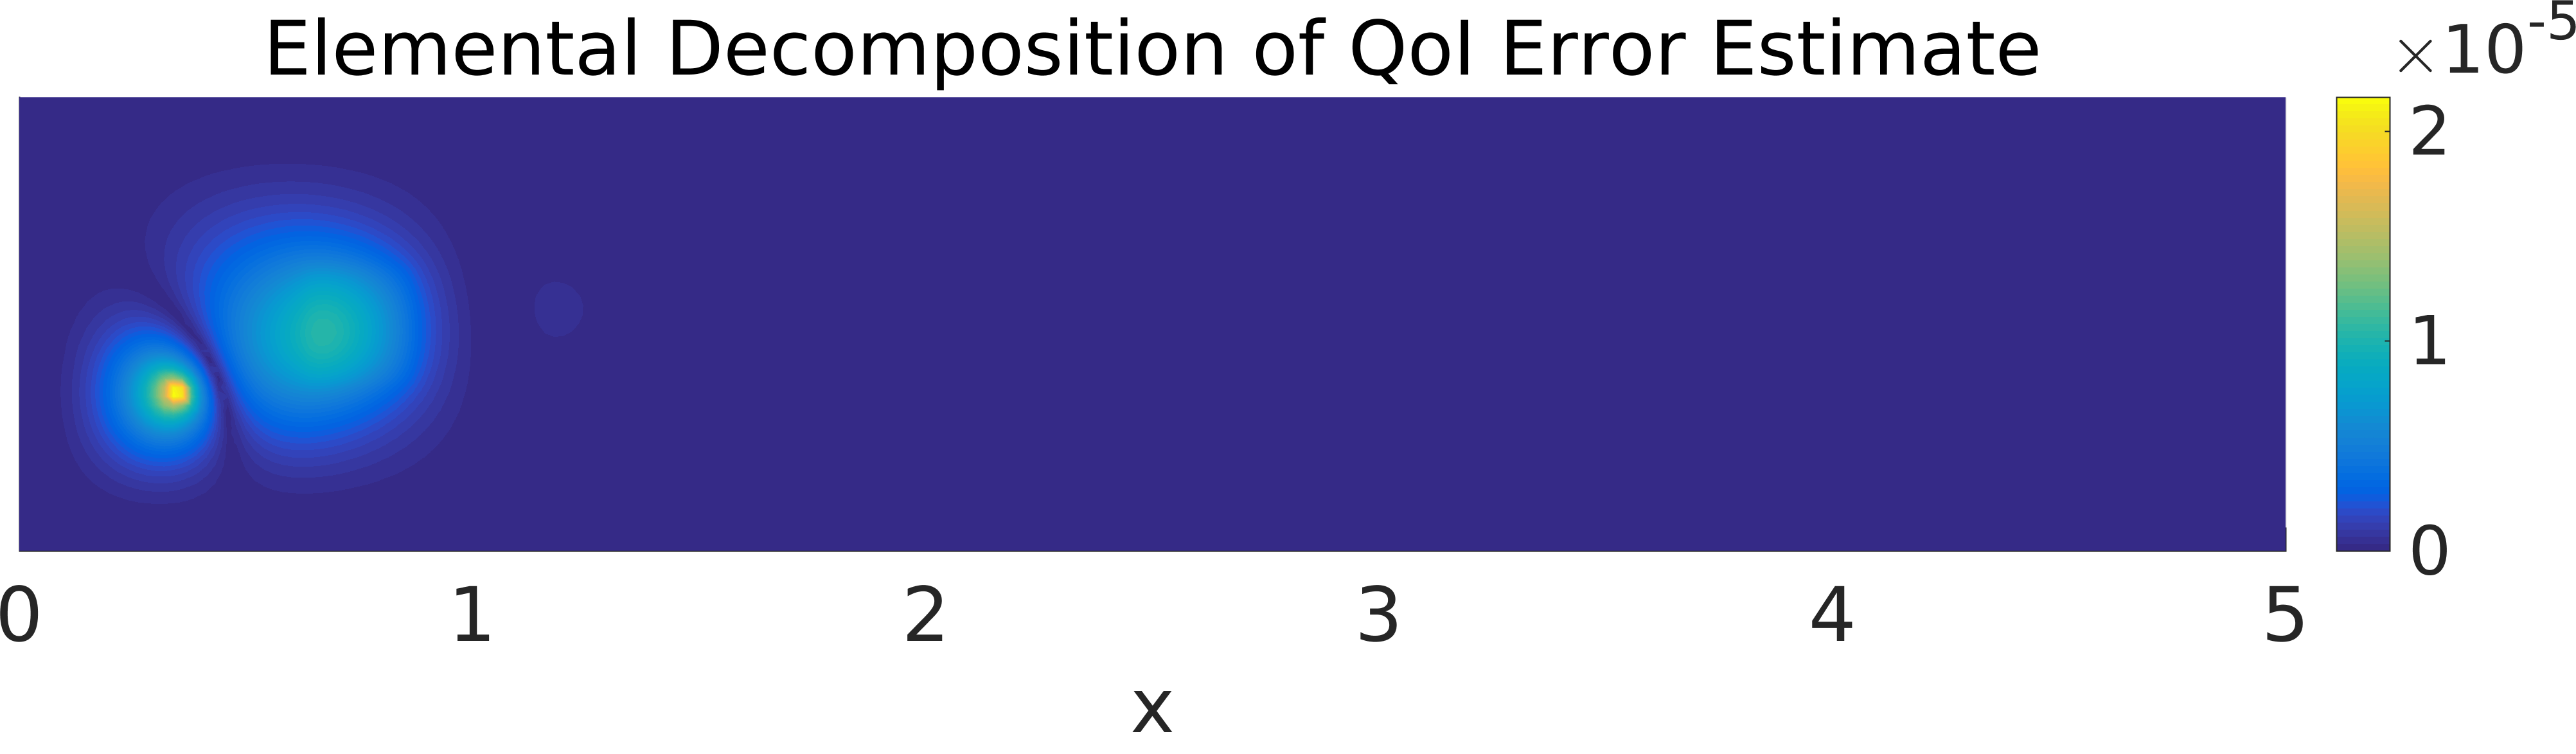
\includegraphics[width=0.51\textwidth]{baseSeries/err_breakdown_LF.png}
    \vspace{-0.5\baselineskip}
    \caption{MF$_0$ ($0\%$ HF)}
    \label{fig:baseRef0}
    \vspace{0.8\baselineskip}
  \end{subfigure}
	\begin{subfigure}[b]{\textwidth}
  \centering
    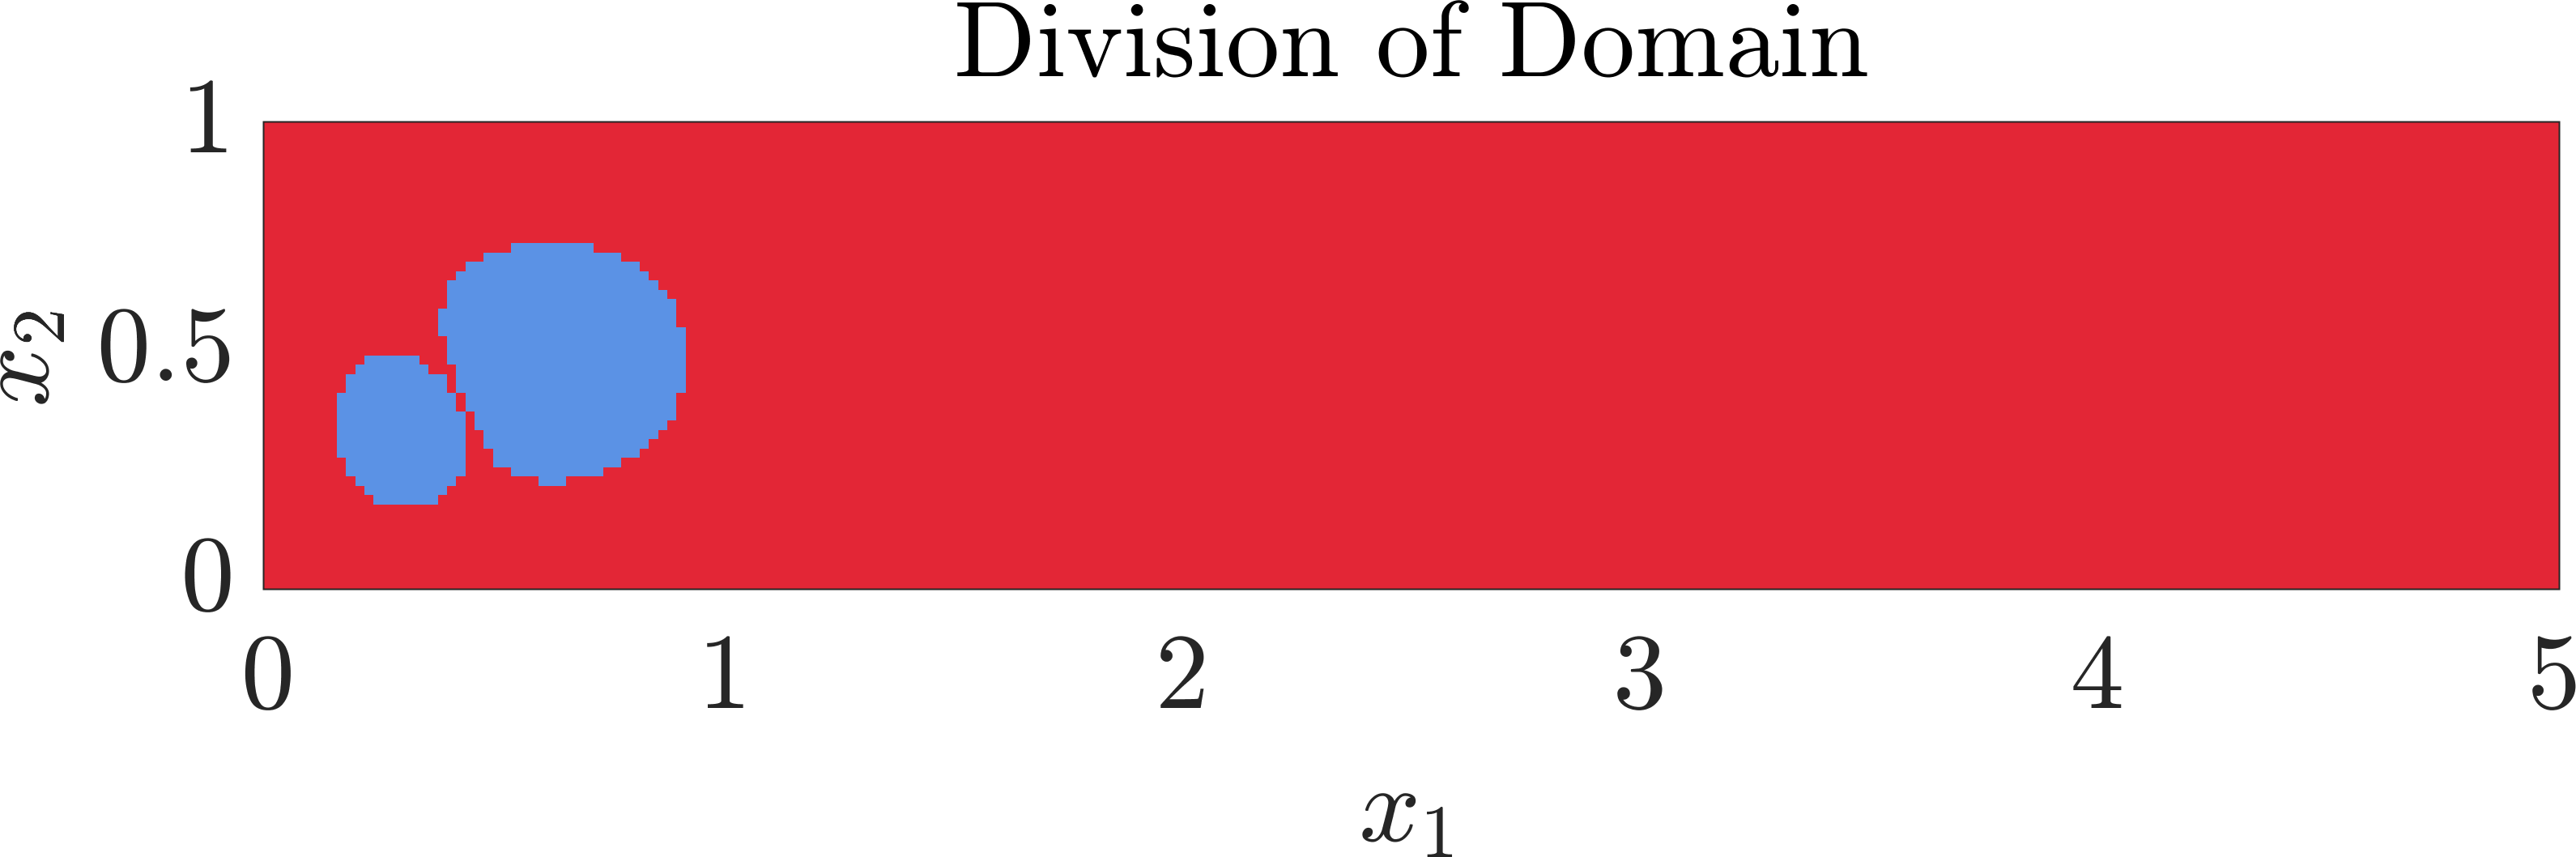
\includegraphics[width=0.48\textwidth]{baseSeries/cd_cdr_MF01_divvy.png}
    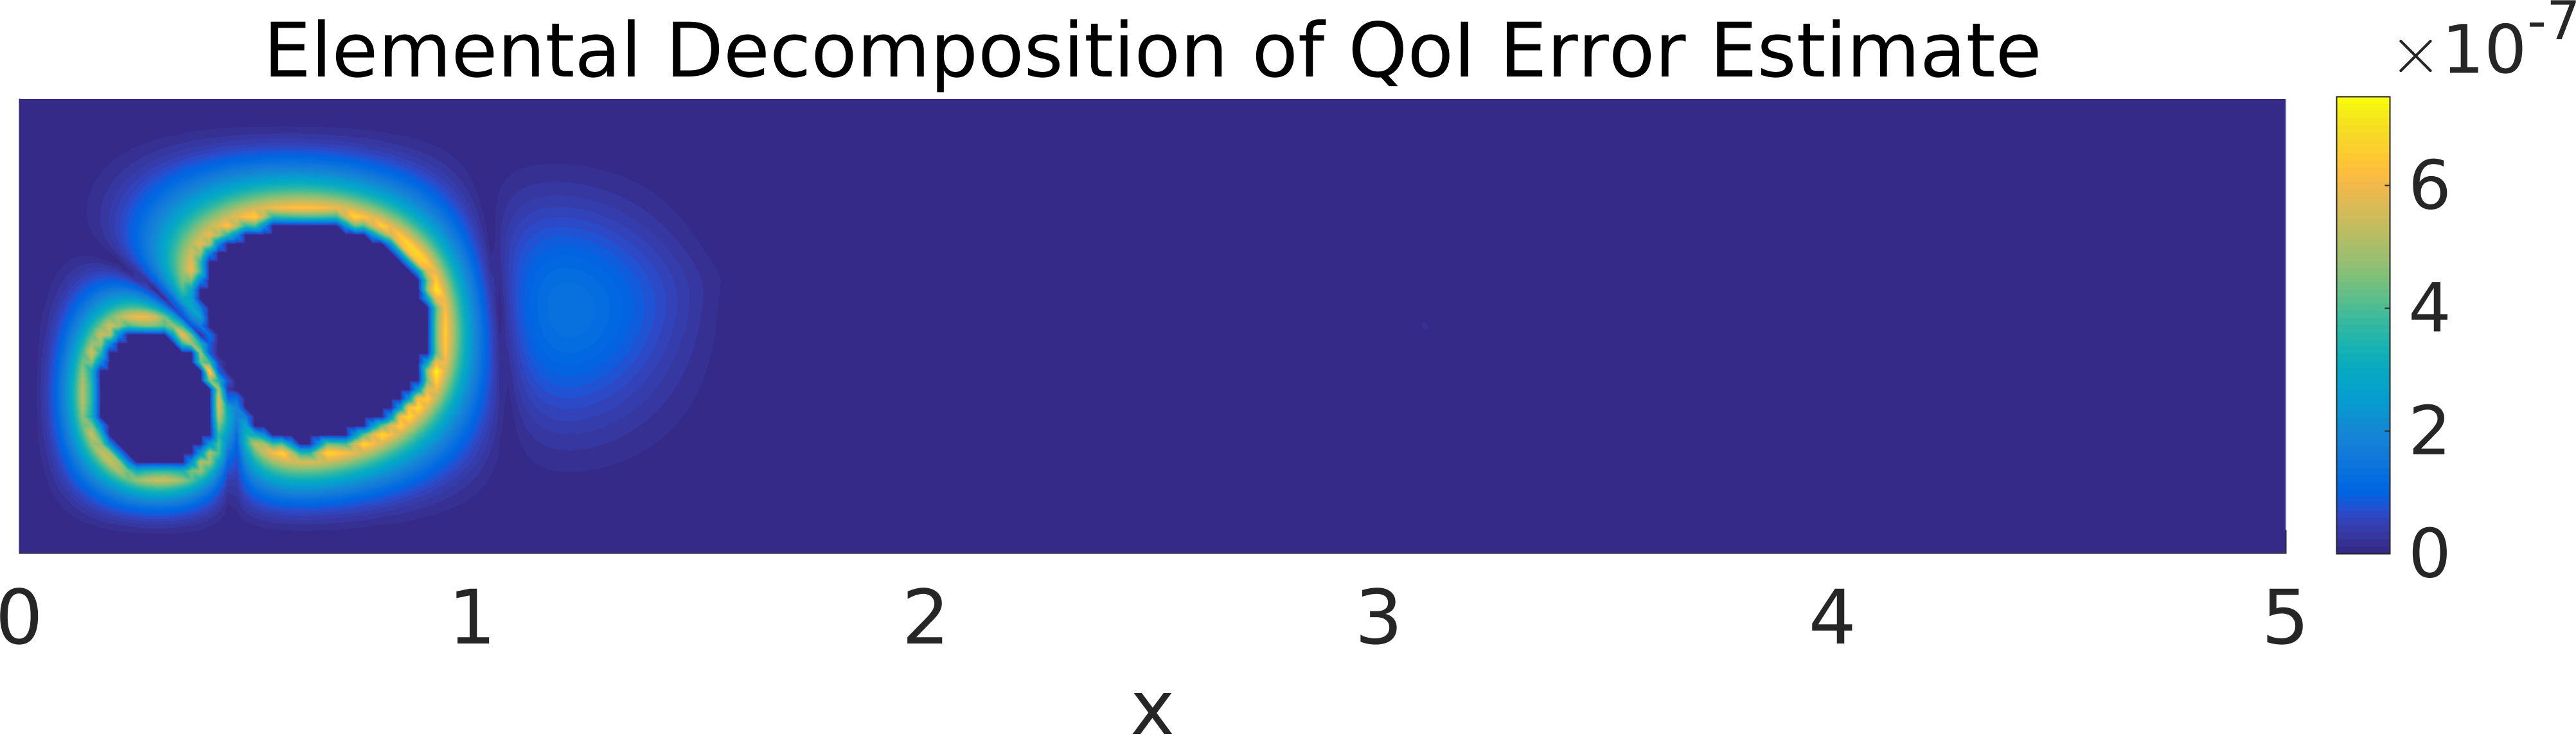
\includegraphics[width=0.51\textwidth]{baseSeries/err_breakdown_MF01.png}
    \vspace{-0.5\baselineskip}
    \caption{MF$_1$ ($5\%$ HF)}
    \vspace{0.8\baselineskip}
  \end{subfigure}
  \begin{subfigure}[b]{\textwidth}
  \centering
    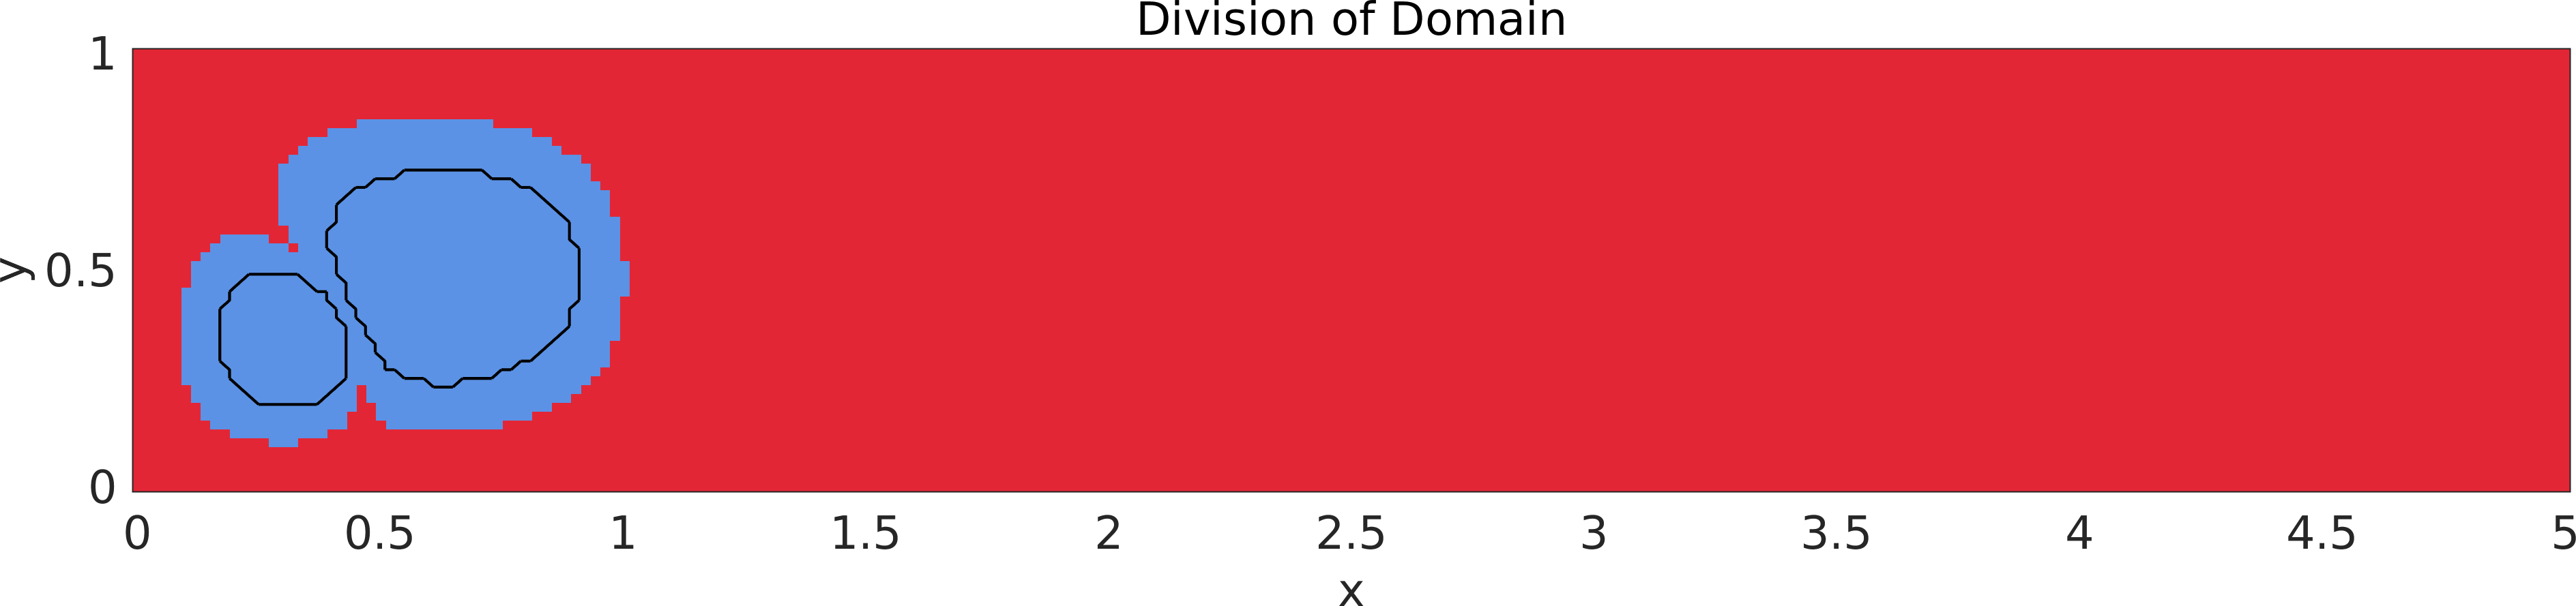
\includegraphics[width=0.48\textwidth]{baseSeries/cd_cdr_MF02_divvy.png}
    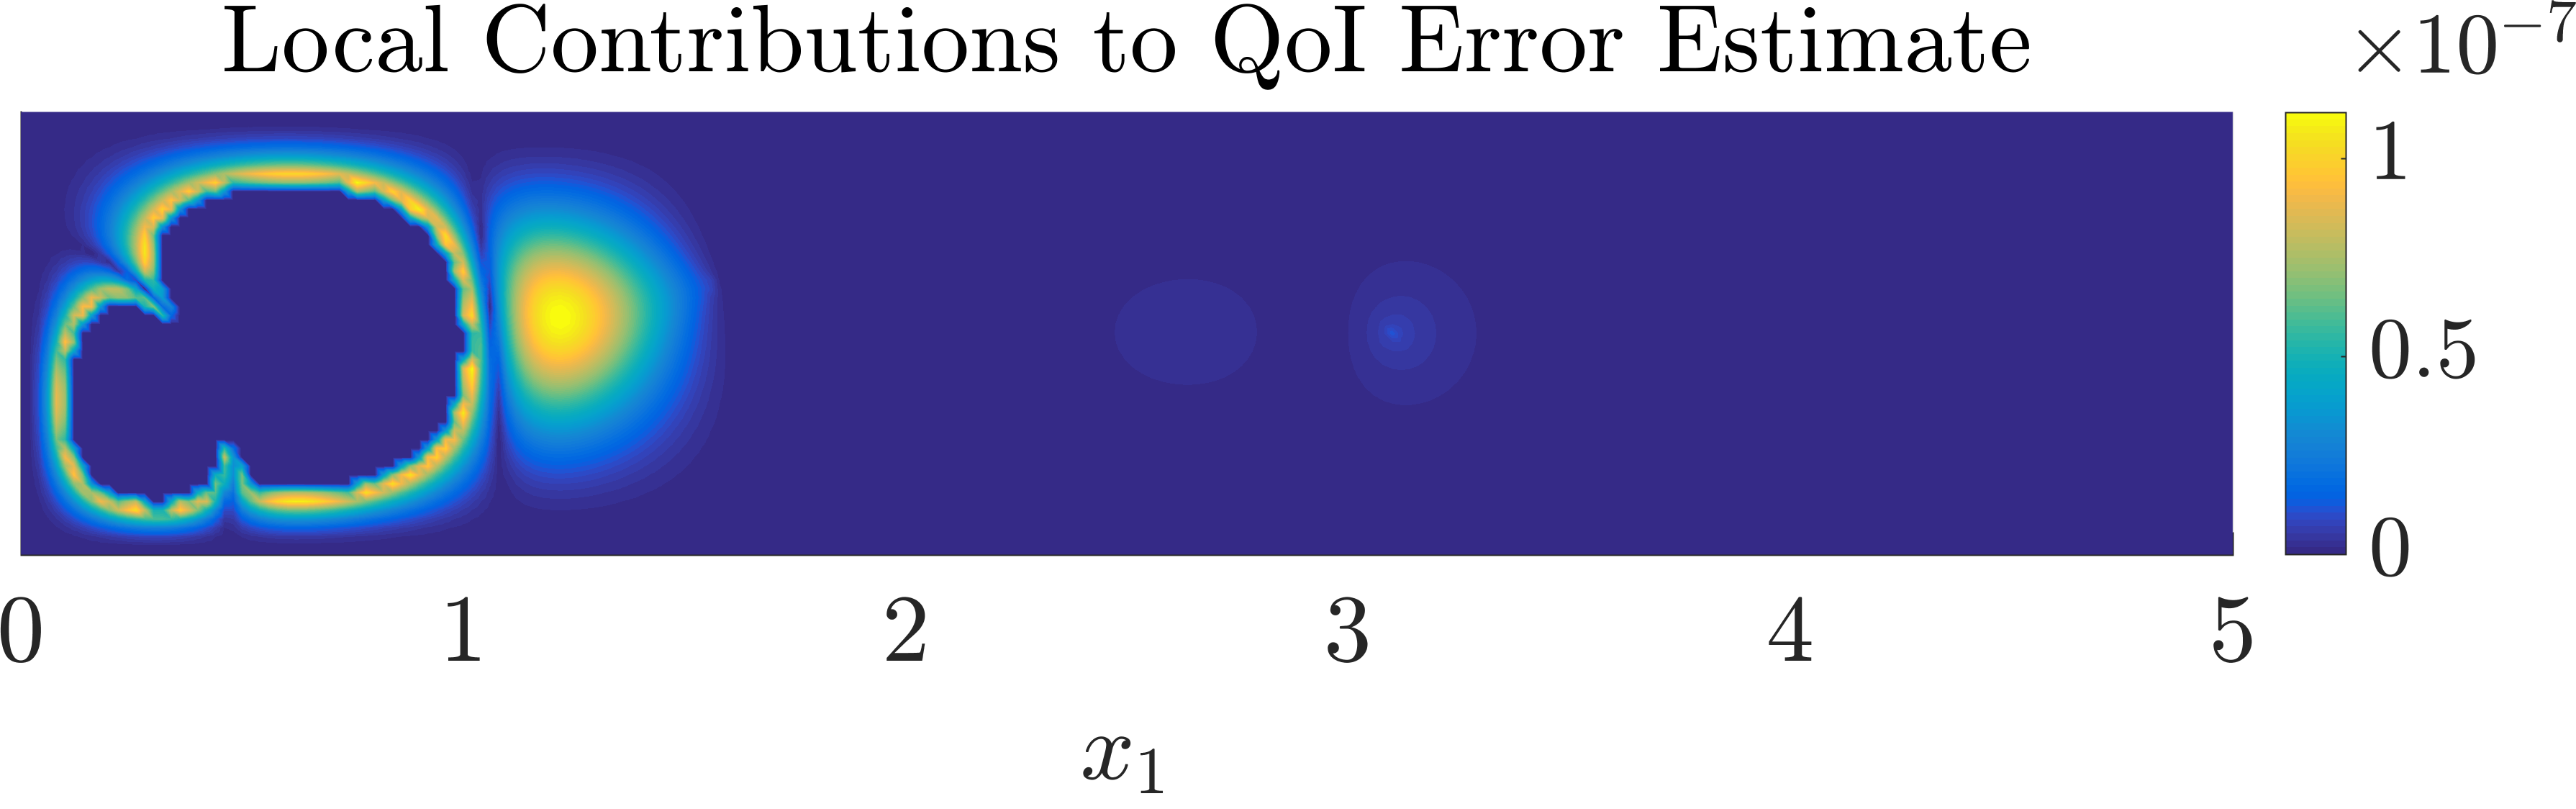
\includegraphics[width=0.51\textwidth]{baseSeries/err_breakdown_MF02.png}
    \vspace{-0.5\baselineskip}
    \caption{MF$_2$ ($10\%$ HF)}
    \vspace{0.8\baselineskip}
  \end{subfigure}
\caption{Local error contributions (right) and domain division (left; low-fidelity convection-diffusion model used in red portion, high-fidelity convection-diffusion-reaction model used in blue portion) for mixed-fidelity models.}
\label{fig:baseRef}
\end{figure}
%
Note that the error contribution of each basis function whose support is entirely within the high-fidelity regions is zero.

We see that the largest local error contribution is concentrated in the QoI region, and the data point closest to the QoI. In the first decomposition of the error (Figure~\ref{fig:baseRef0}), the region where the elemental error is maximum is the leftmost data point. Since the constraining model is an elliptic PDE, with a weak convection, information flow is localized, and is weakly convected from left to right. Therefore, for the calculation of the QoI, it is most important to refine the region near the leftmost data point, and the QoI region. After that, the error decomposition suggests refinement in regions upstream and around the middle data point, and then the rightmost data point.

Figure~\ref{fig:baseErr} shows the true and estimated absolute relative errors in the QoI for the various mixed-fidelity models generated by Algorithm~\ref{alg:refSeries}. In this case, we see that the QoI error of only $1\%$ is attained with a mixed-fidelity model where the high-fidelity model is used in only about $10\%$ of the domain. We note that there is no guarantee that either the error in the QoI or the relative error in the error estimate will decrease monotonically as more of the domain is refined.
%
\begin{figure}[h]
\centering
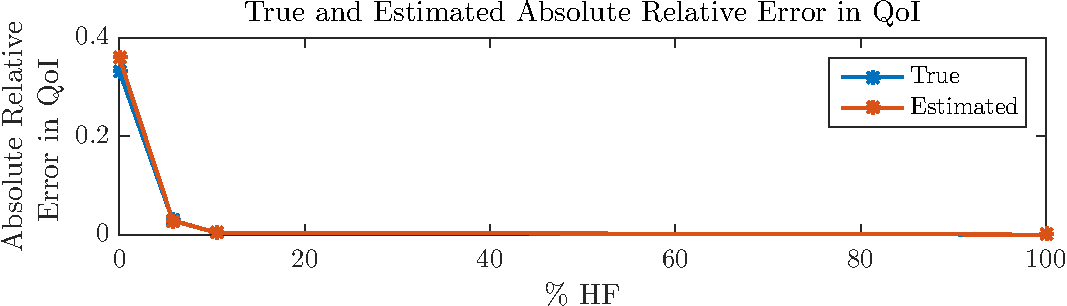
\includegraphics[width=0.7\textwidth]{baseSeries/err_est.pdf}
\caption{True and estimated absolute relative error in QoI, plotted as a function of the percentage area of the domain in which the high-fidelity convection-diffusion-reaction model is used.\red{does this even have enough points to warrant a graph? or would a table be better?}}
\label{fig:baseErr}
\end{figure}
%

%------------------------------------------------------------%
\subsubsection{Interaction of Observations and QoI} \label{sec:qoivdata}
%------------------------------------------------------------%
%
The error estimate decomposition (\ref{eq:basisblame}) suggests the use of the high-fidelity model in areas of the domain that are important to the interaction of the observations and QoI; the interaction of these two can be complex, and the areas suggested for refinement may be nonintuitive. To see this, we compare the error estimate decomposition for three sizes of the QoI region $\Omega_I$ given the same set of data points, and for three nested sets of data points given the same QoI region. For the sake of illustration, we make two refinement iterations for each combination of observations and QoI region, regardless of the magnitude of the relative error estimate. However, it was noticed that the number of iterations needed to achieve a given tolerance increased as the QoI region increased, but did not consistently increase or decrease with the number of data points.

The error decomposition for three increasingly large, nested QoI regions $\Omega_I$ given the same set of observations is shown in Figure \ref{fig:qoiStudy}. The bottom row gives the baseline case presented in Section~\ref{sec:cdvcdrBaseRef}, although here the basis functions with the largest $5\%$ of the error are choesn, so the proportion of additional refined elements in each iteration is slightly larger. Although refinement is still most important around the data point closest to $x_1=0$, as the QoI region expands the other two data points become more important in that the error decomposition suggests refinement around them earlier. As the QoI region expands, it is also more clearly noticeable that refinement is not equally important in all parts of the QoI region.

\begin{figure}
\captionsetup[subfigure]{justification=centering}
\centering
  \begin{subfigure}[t]{0.20\textwidth}
  \centering
    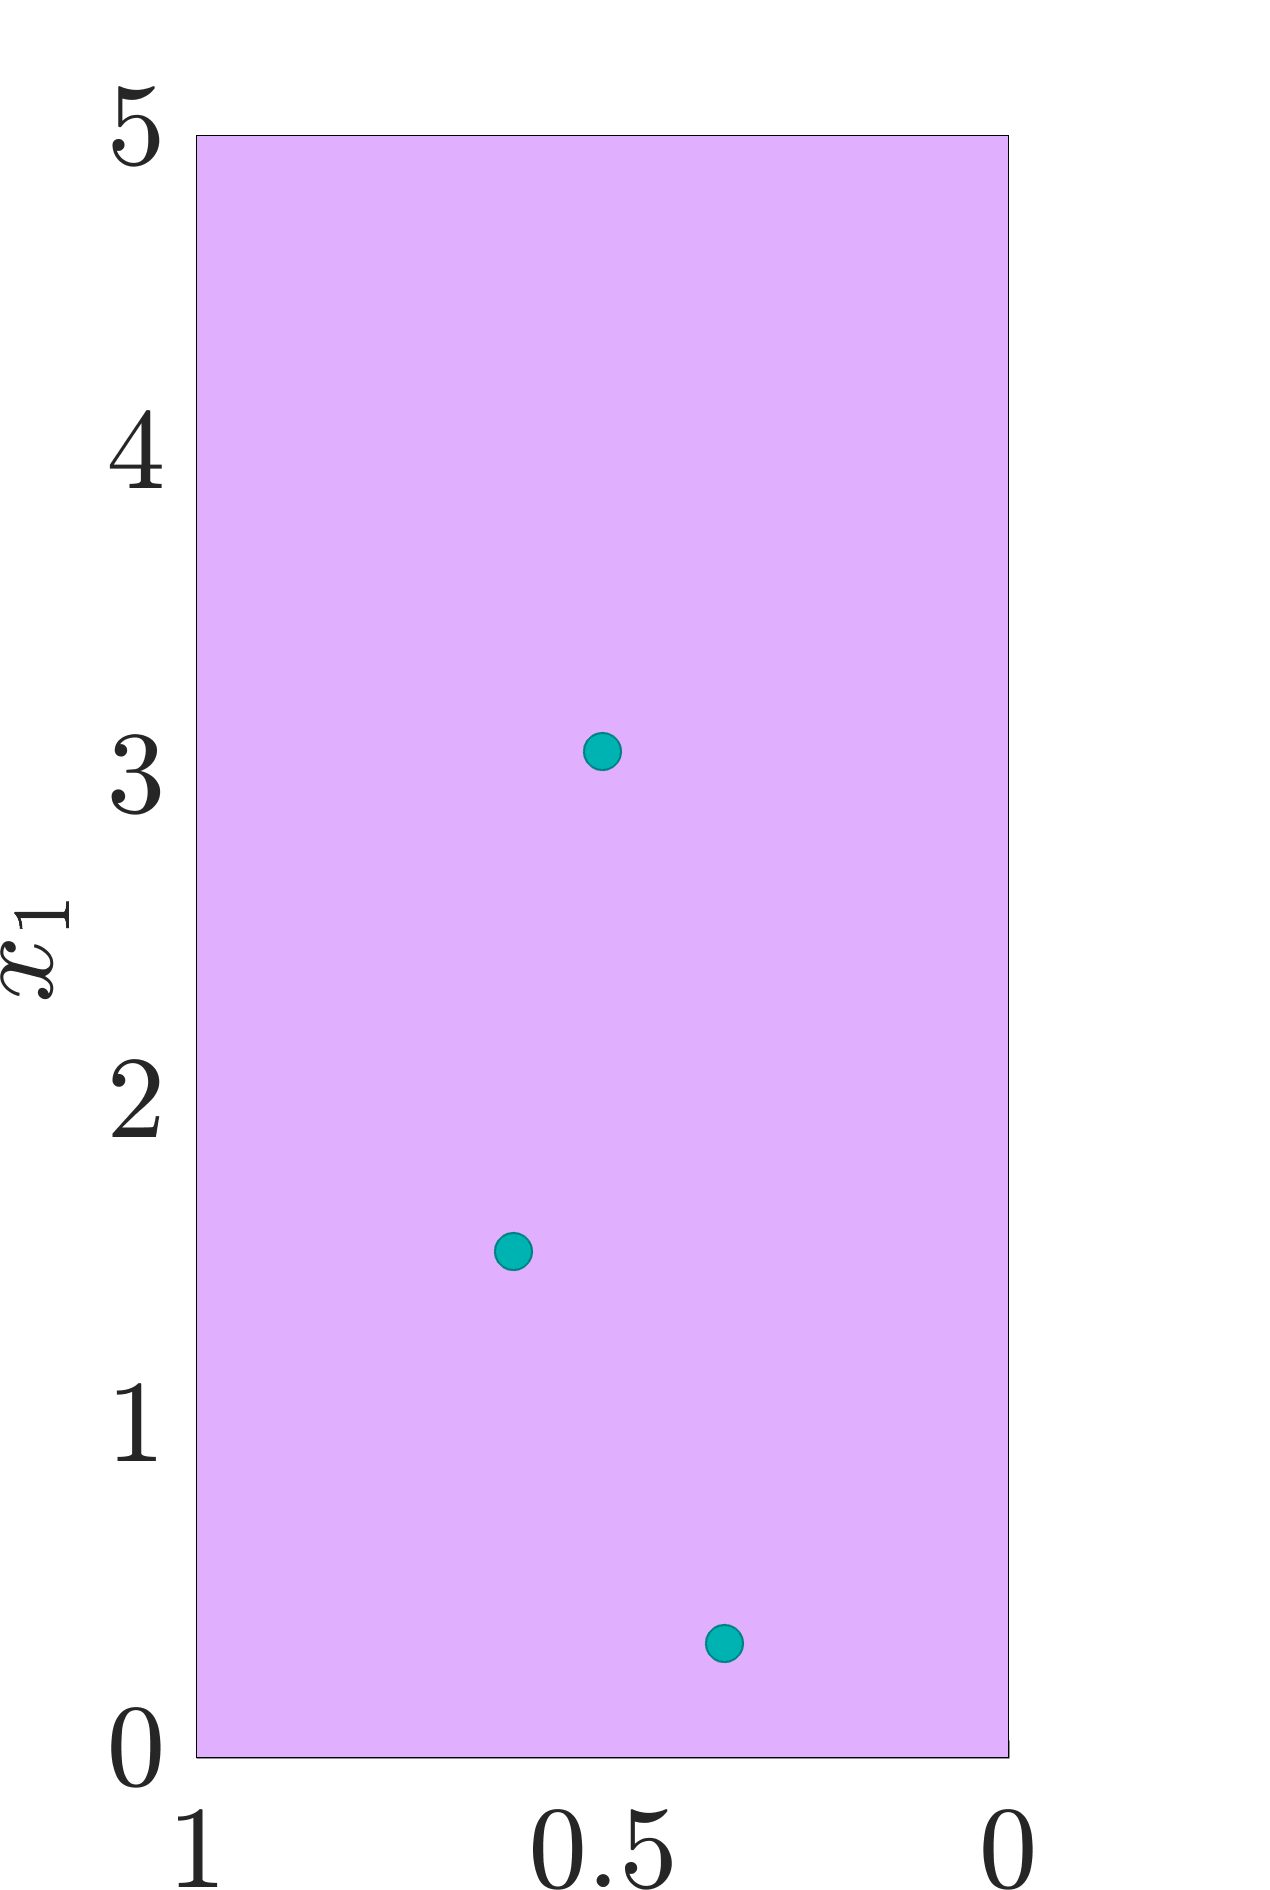
\includegraphics[width=\textwidth]{vs_qoi/qoi5_sens3/setup_5_3.png}
    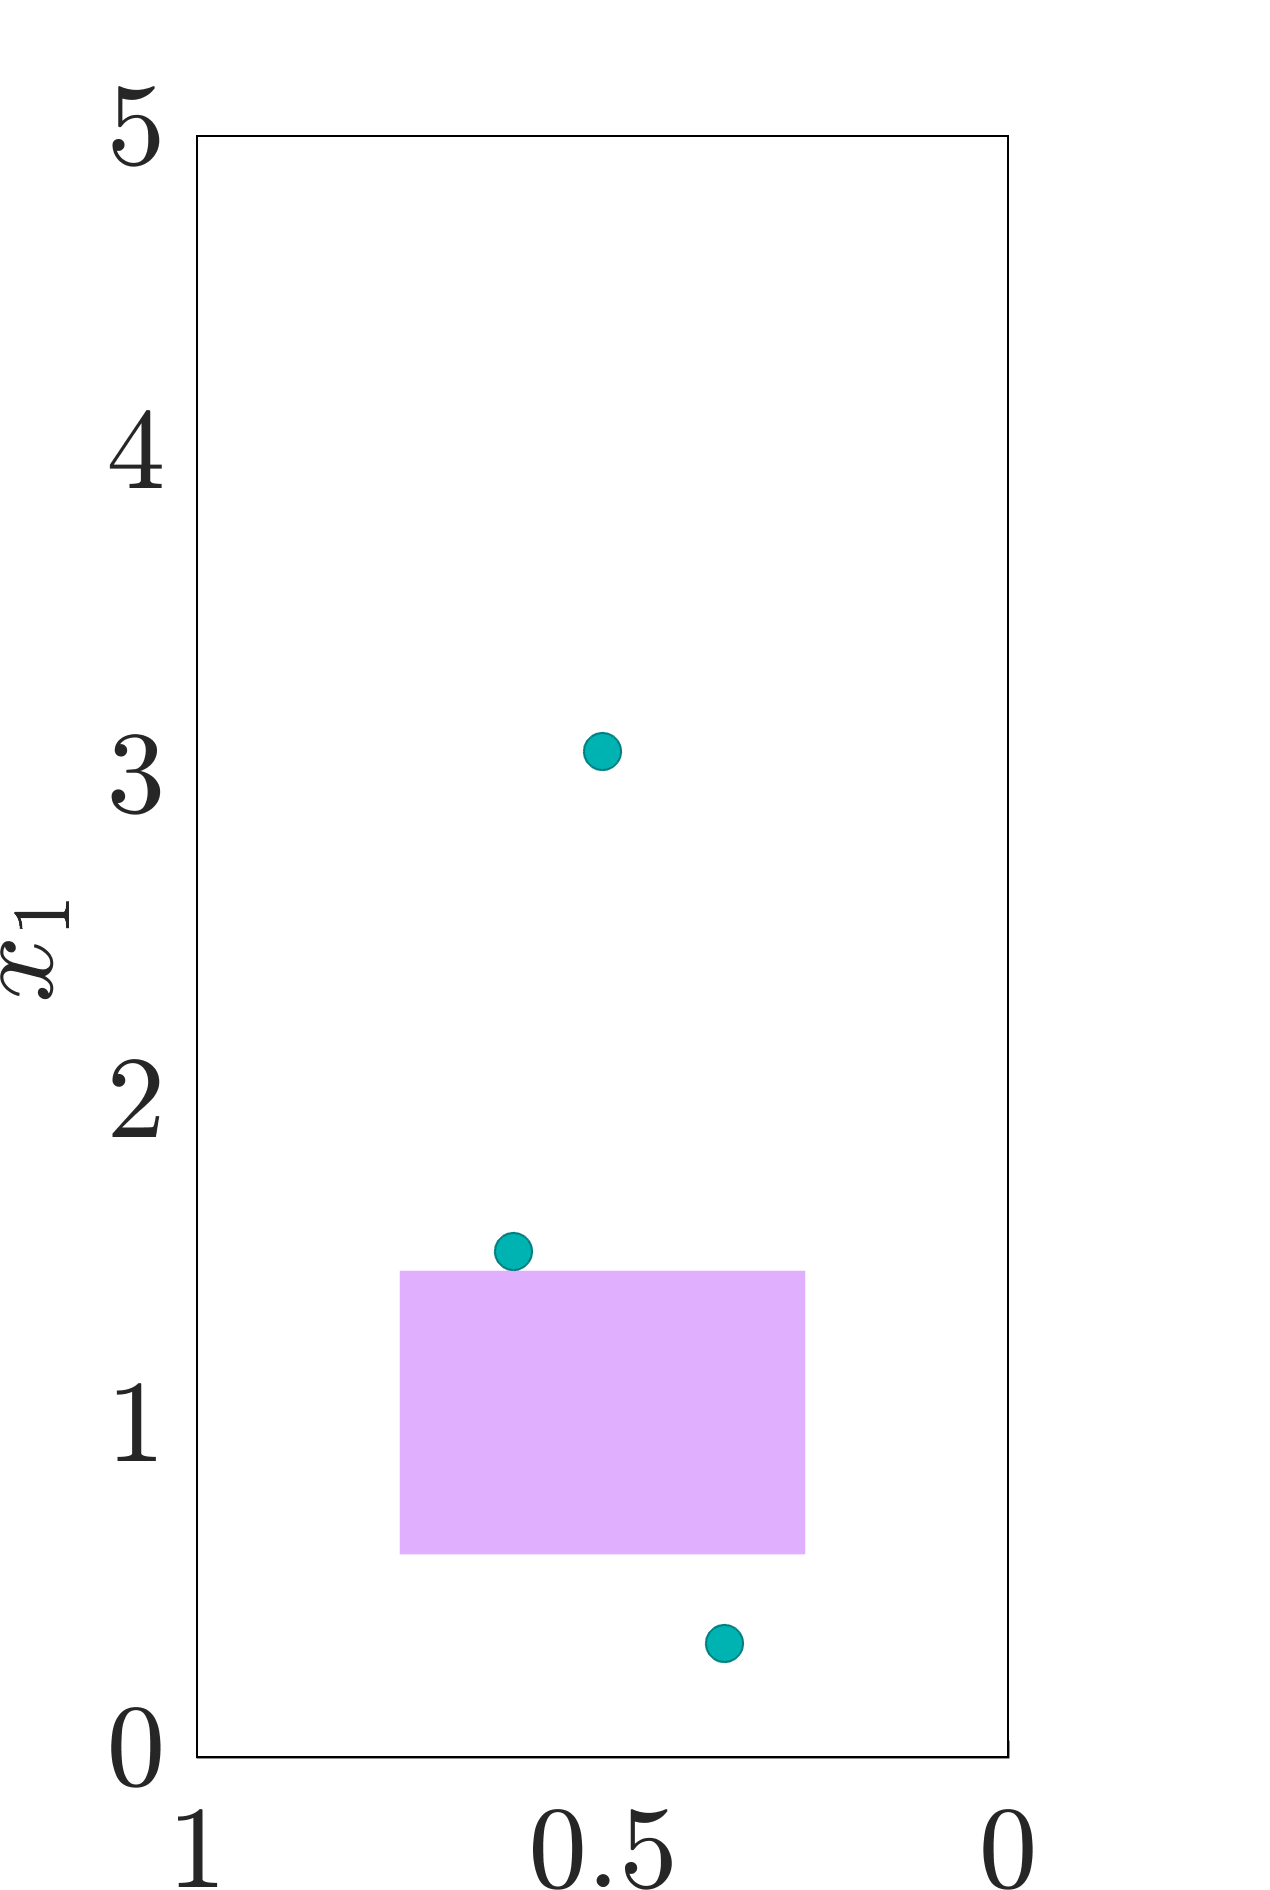
\includegraphics[width=\textwidth]{vs_qoi/qoi7_sens3/setup_7_3.png}
    \includegraphics[width=\textwidth]{vs_qoi/qoi3_sens3/setup_3_3.png}
    \caption{Locations of observations and QoI region $\Omega_I$}
    \label{subfig:obsSetup}
  \end{subfigure}
  \begin{subfigure}[t]{0.20\textwidth}
  \centering
    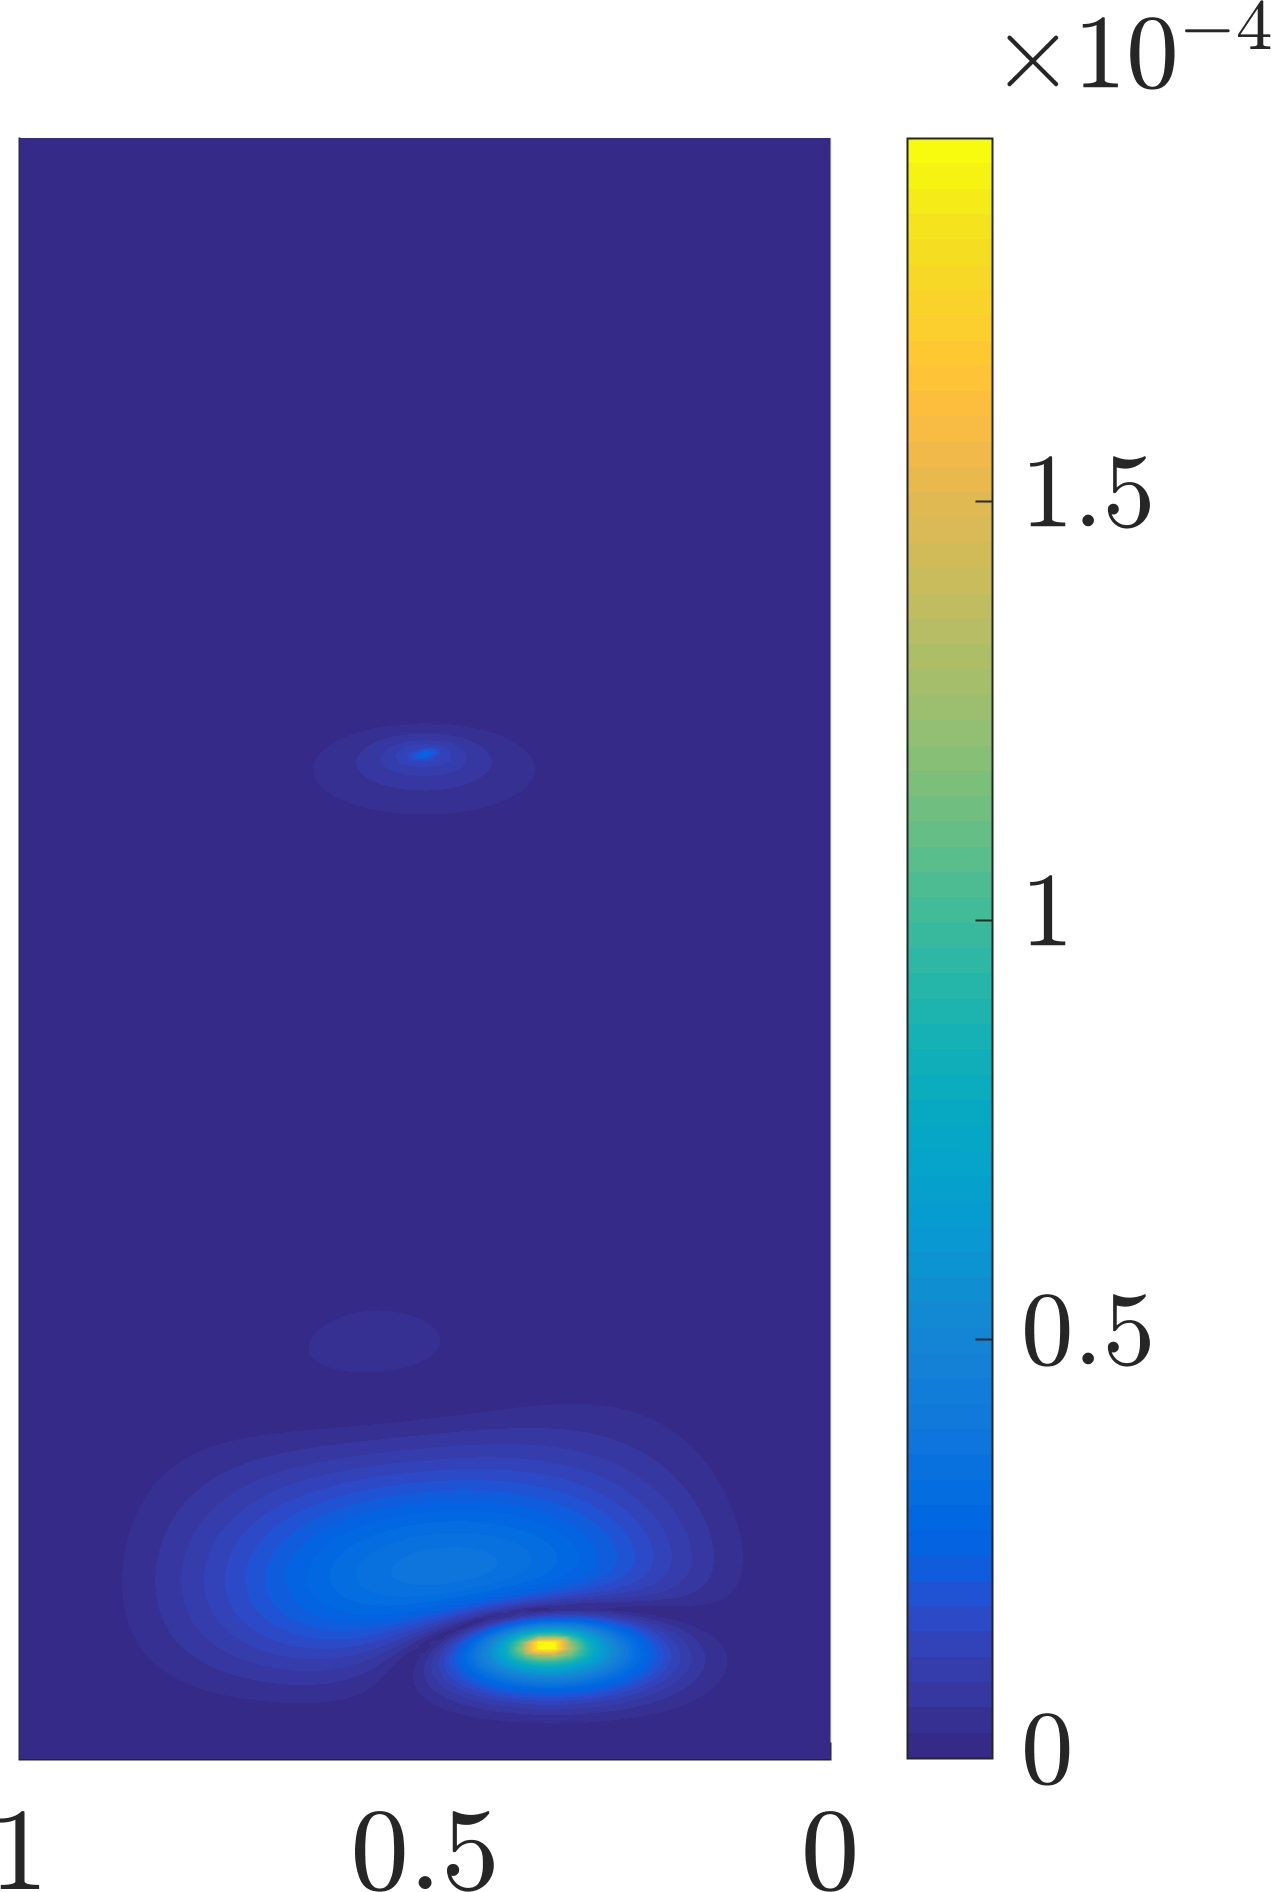
\includegraphics[width=\textwidth]{vs_qoi/qoi5_sens3/err_breakdown_0.png}
    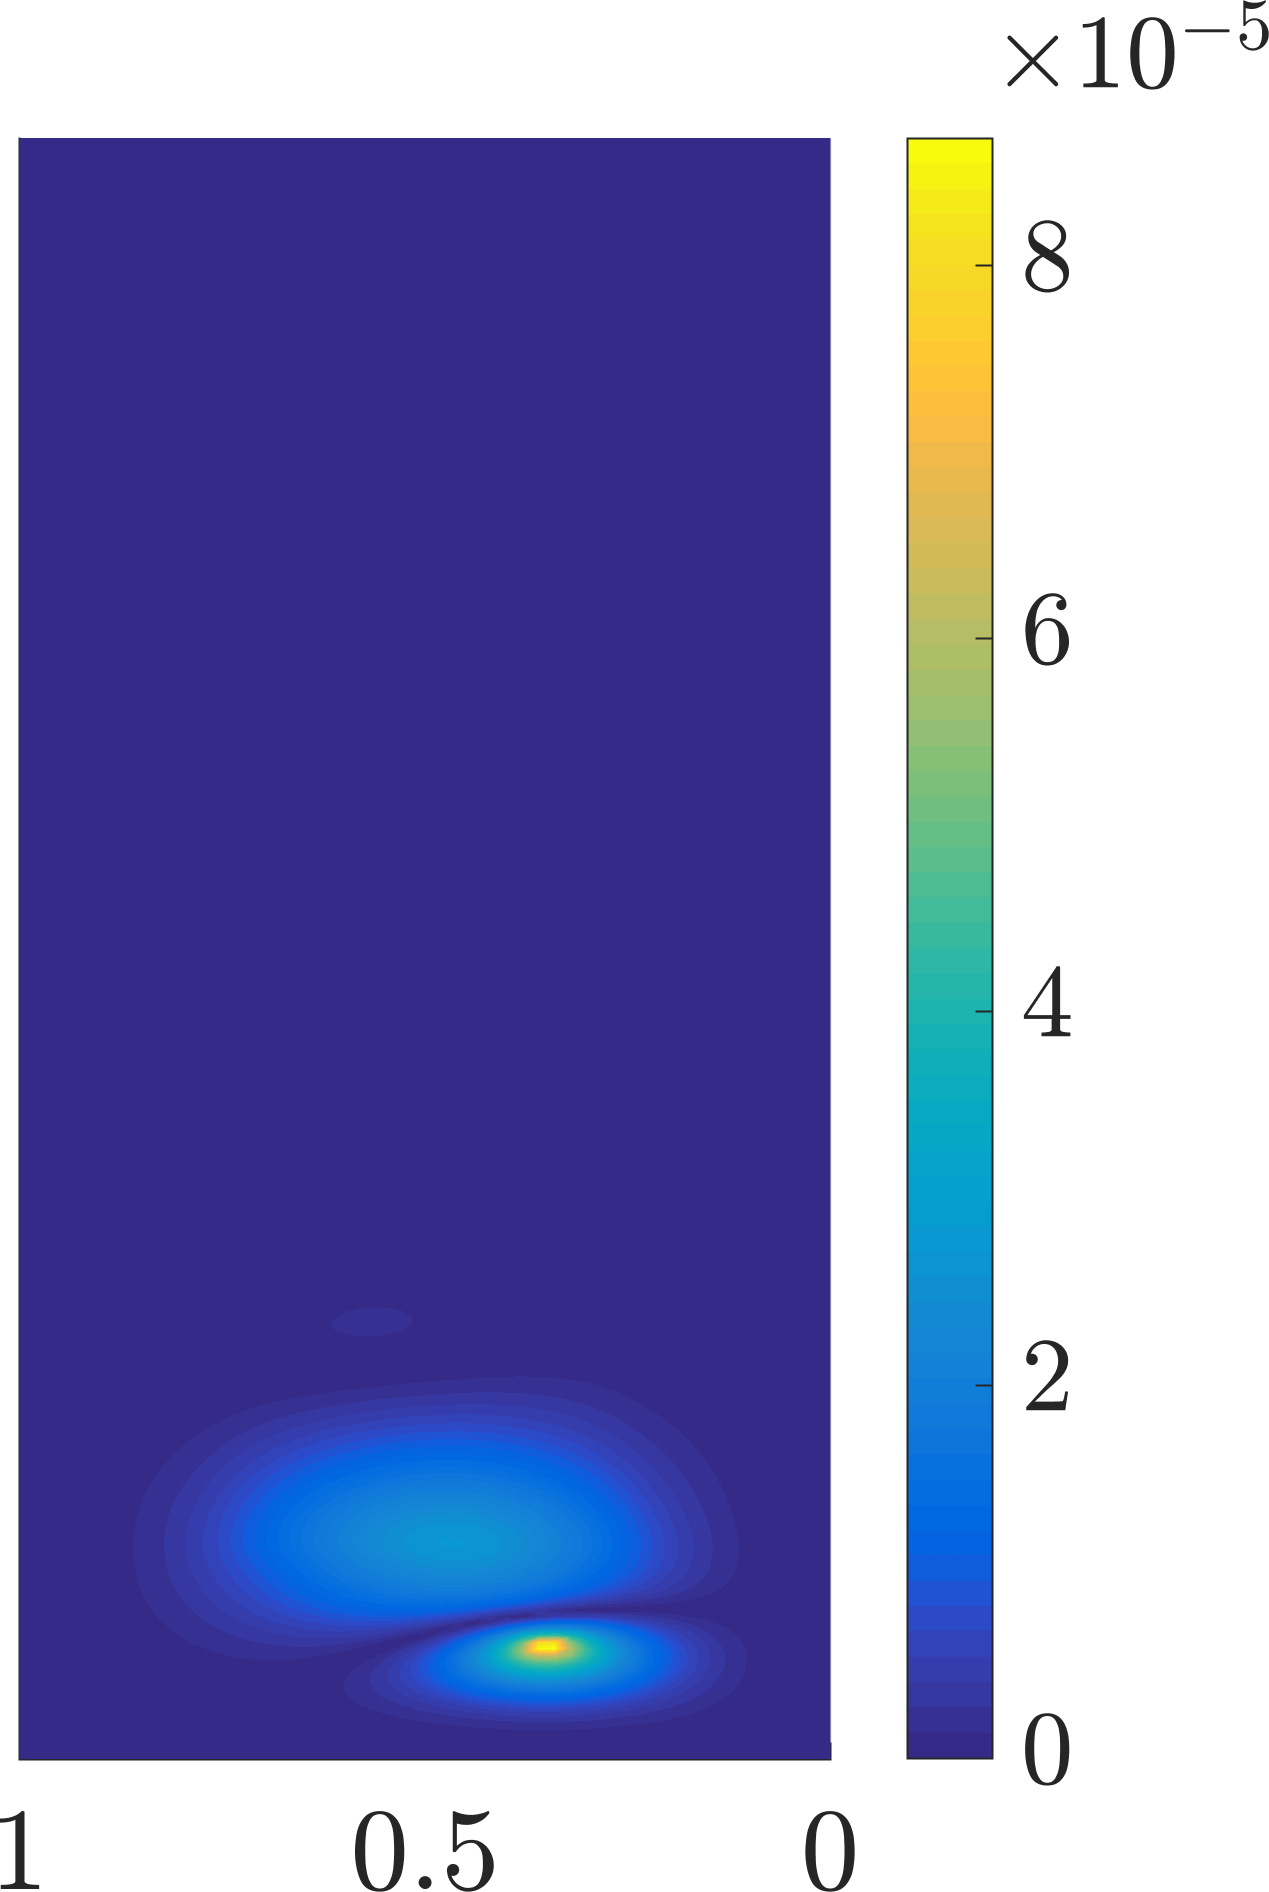
\includegraphics[width=\textwidth]{vs_qoi/qoi7_sens3/err_breakdown_0.png}
    \includegraphics[width=\textwidth]{vs_qoi/qoi3_sens3/err_breakdown_0.png}
    \caption{MF$_0$ \\ ($0\%$ HF)}
    \label{subfig:obsLF}
  \end{subfigure}
  \begin{subfigure}[t]{0.20\textwidth}
  \centering
    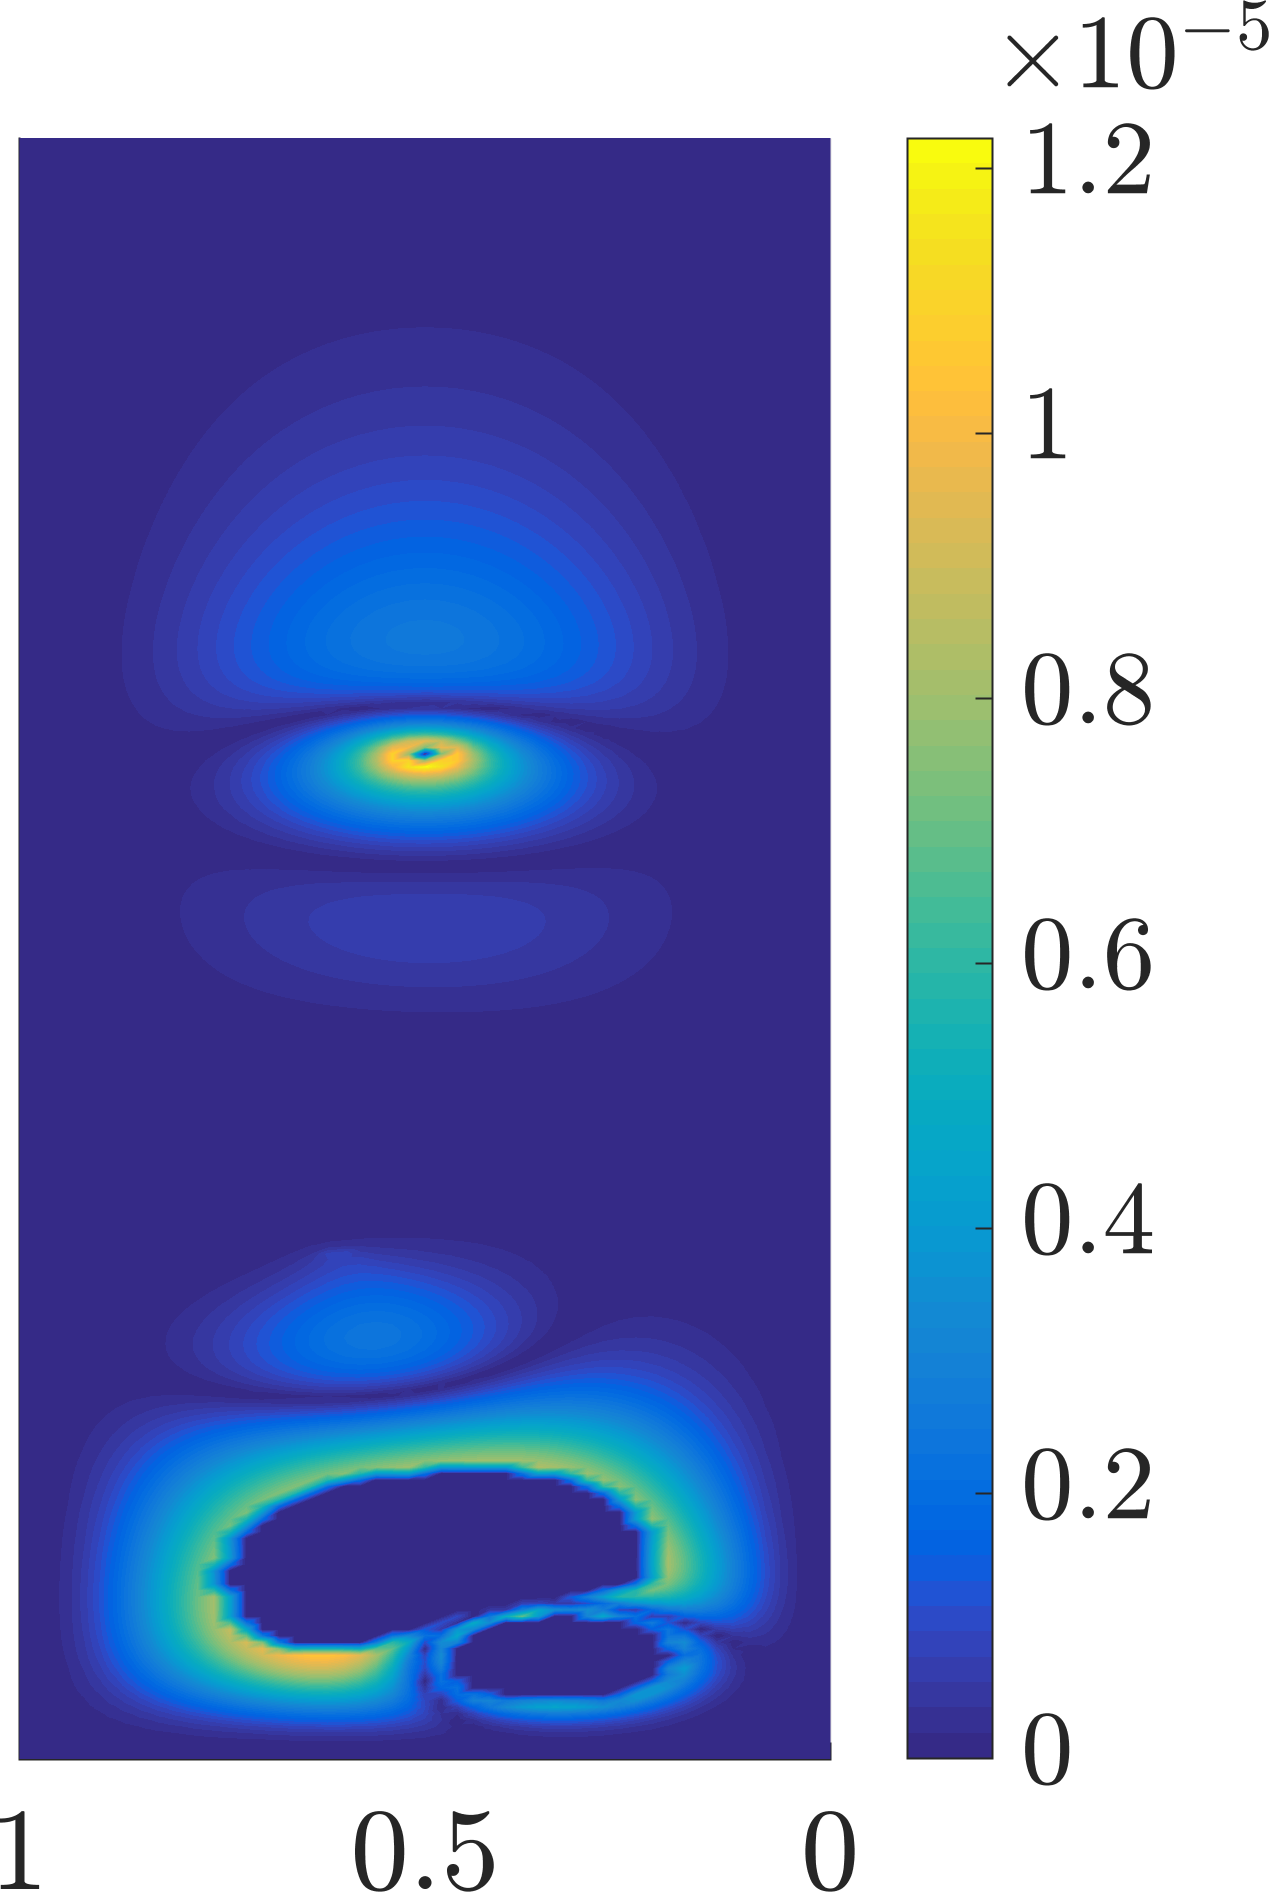
\includegraphics[width=\textwidth]{vs_qoi/qoi5_sens3/err_breakdown_1.png}
    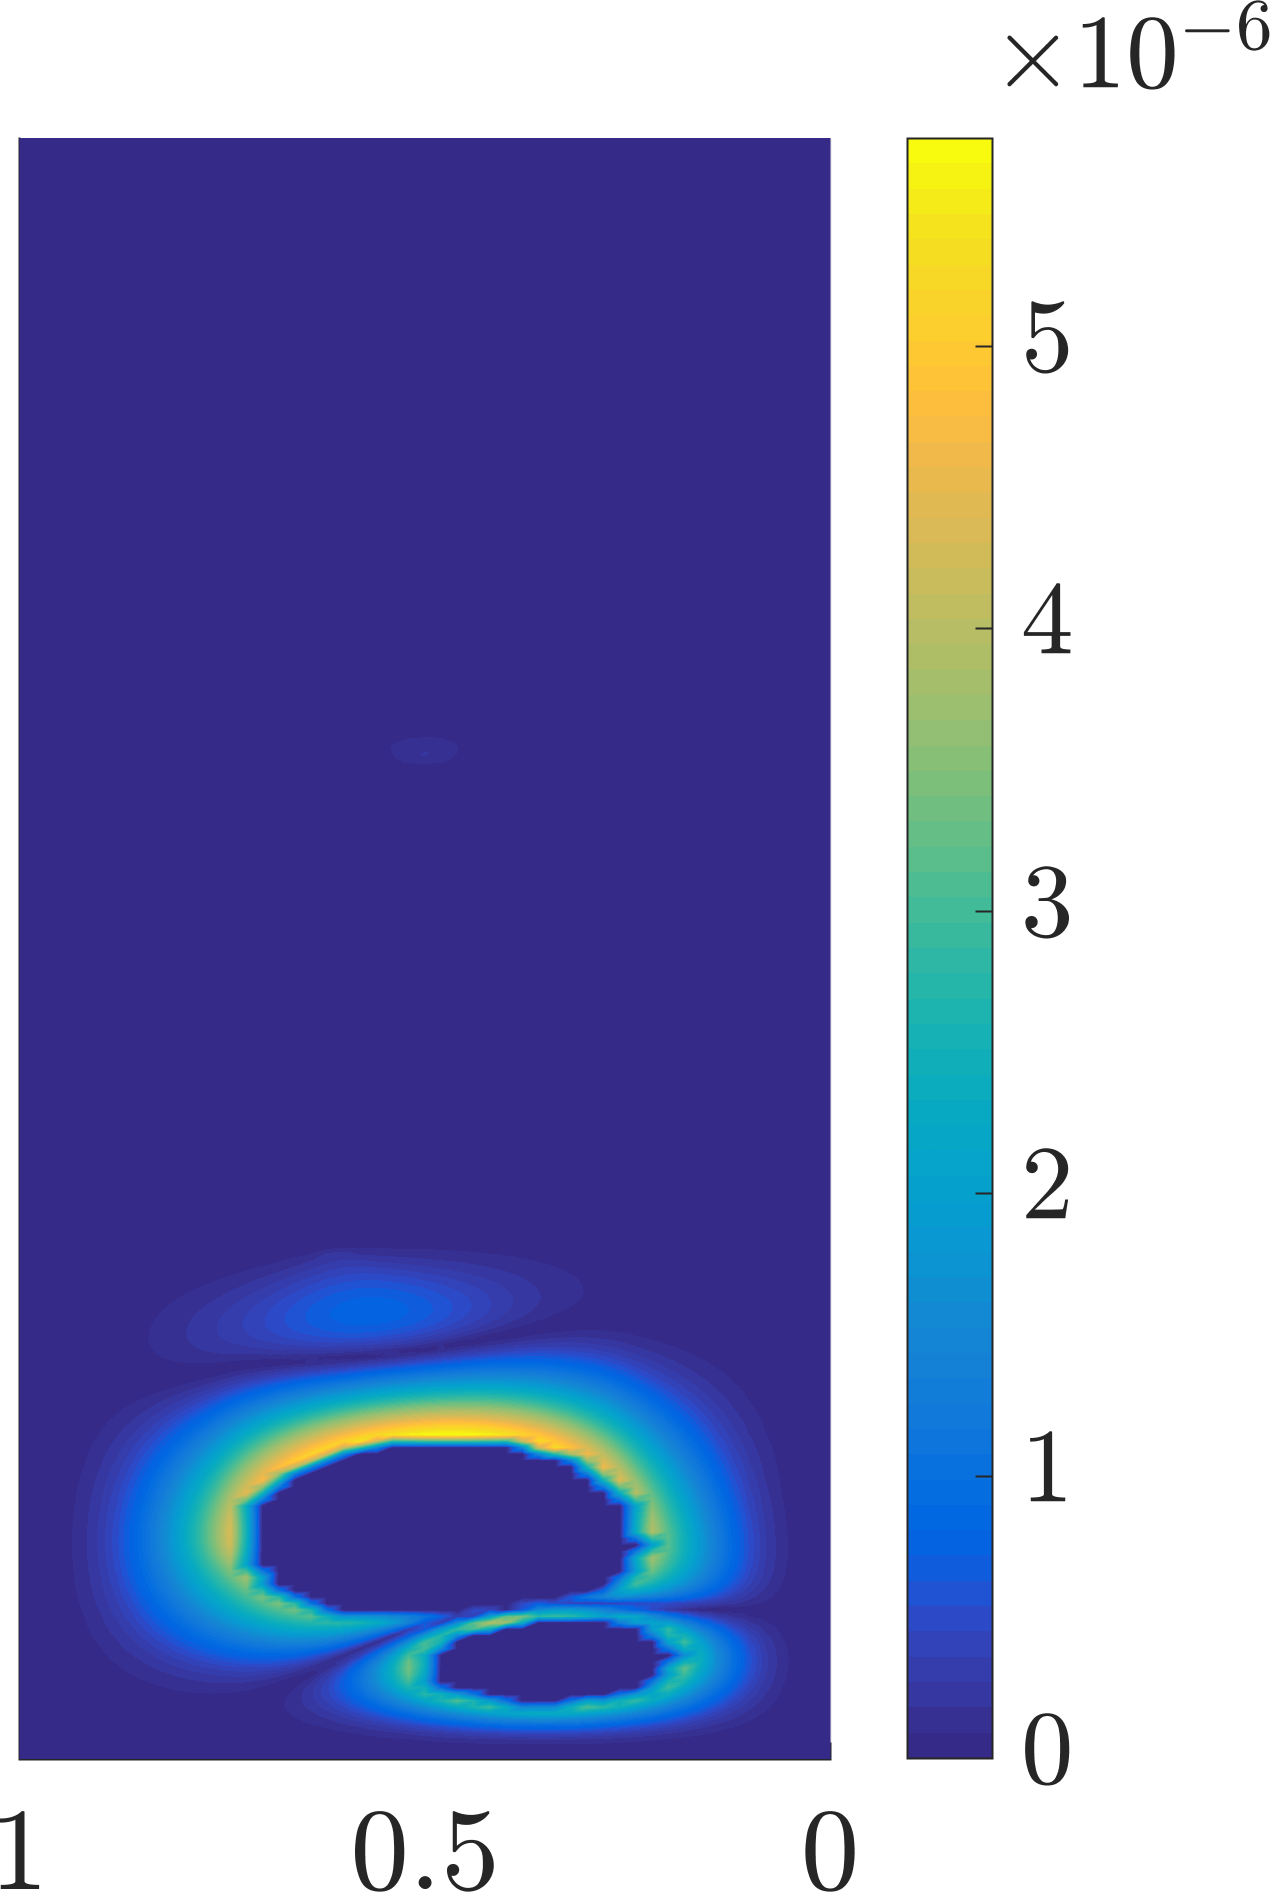
\includegraphics[width=\textwidth]{vs_qoi/qoi7_sens3/err_breakdown_1.png}
    \includegraphics[width=\textwidth]{vs_qoi/qoi3_sens3/err_breakdown_1.png}
    \caption{MF$_1$ \\ ($\sim5\%$ HF)}
  \end{subfigure}
  \begin{subfigure}[t]{0.20\textwidth}
  \centering
    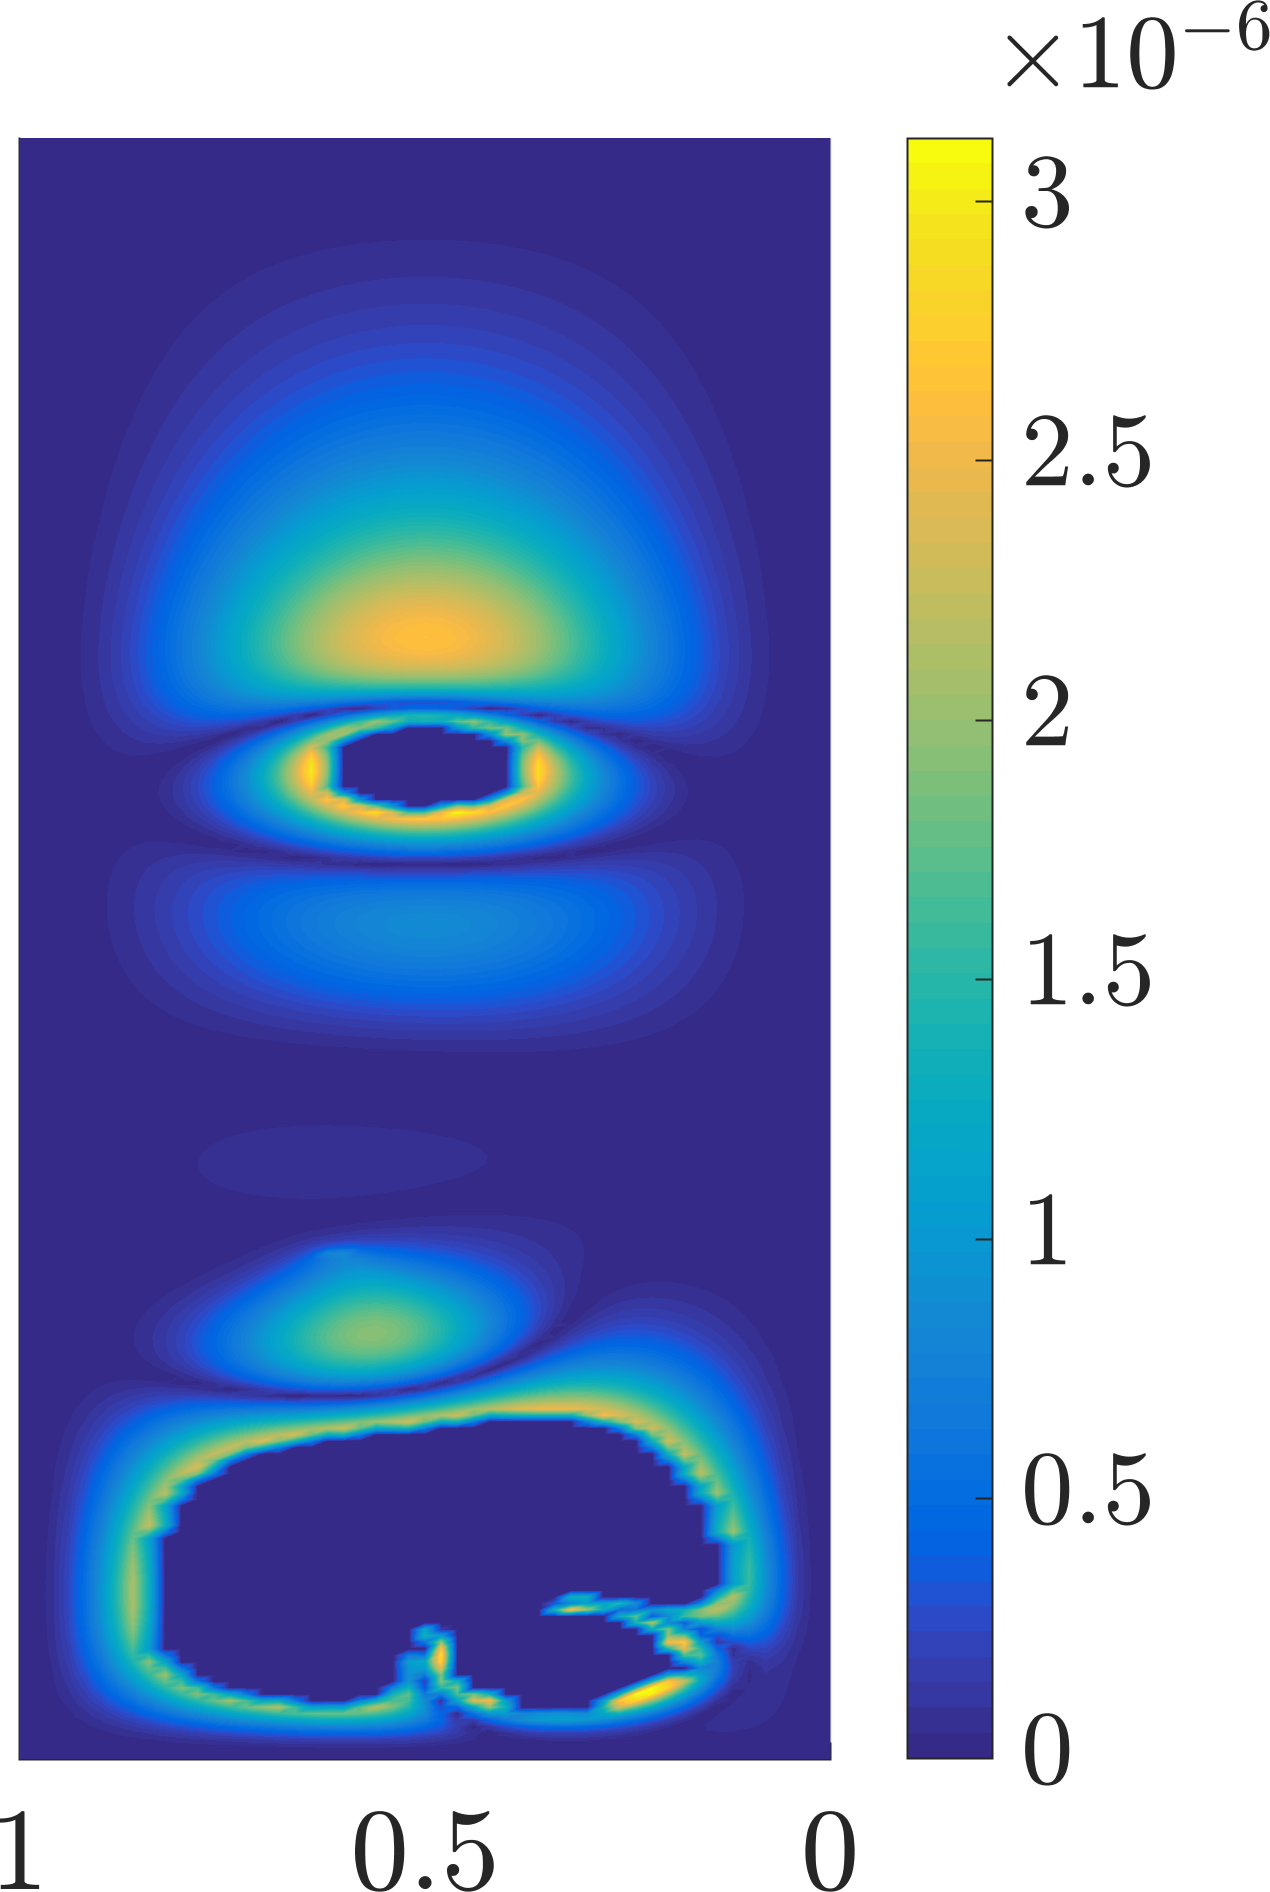
\includegraphics[width=\textwidth]{vs_qoi/qoi5_sens3/err_breakdown_2.png}
    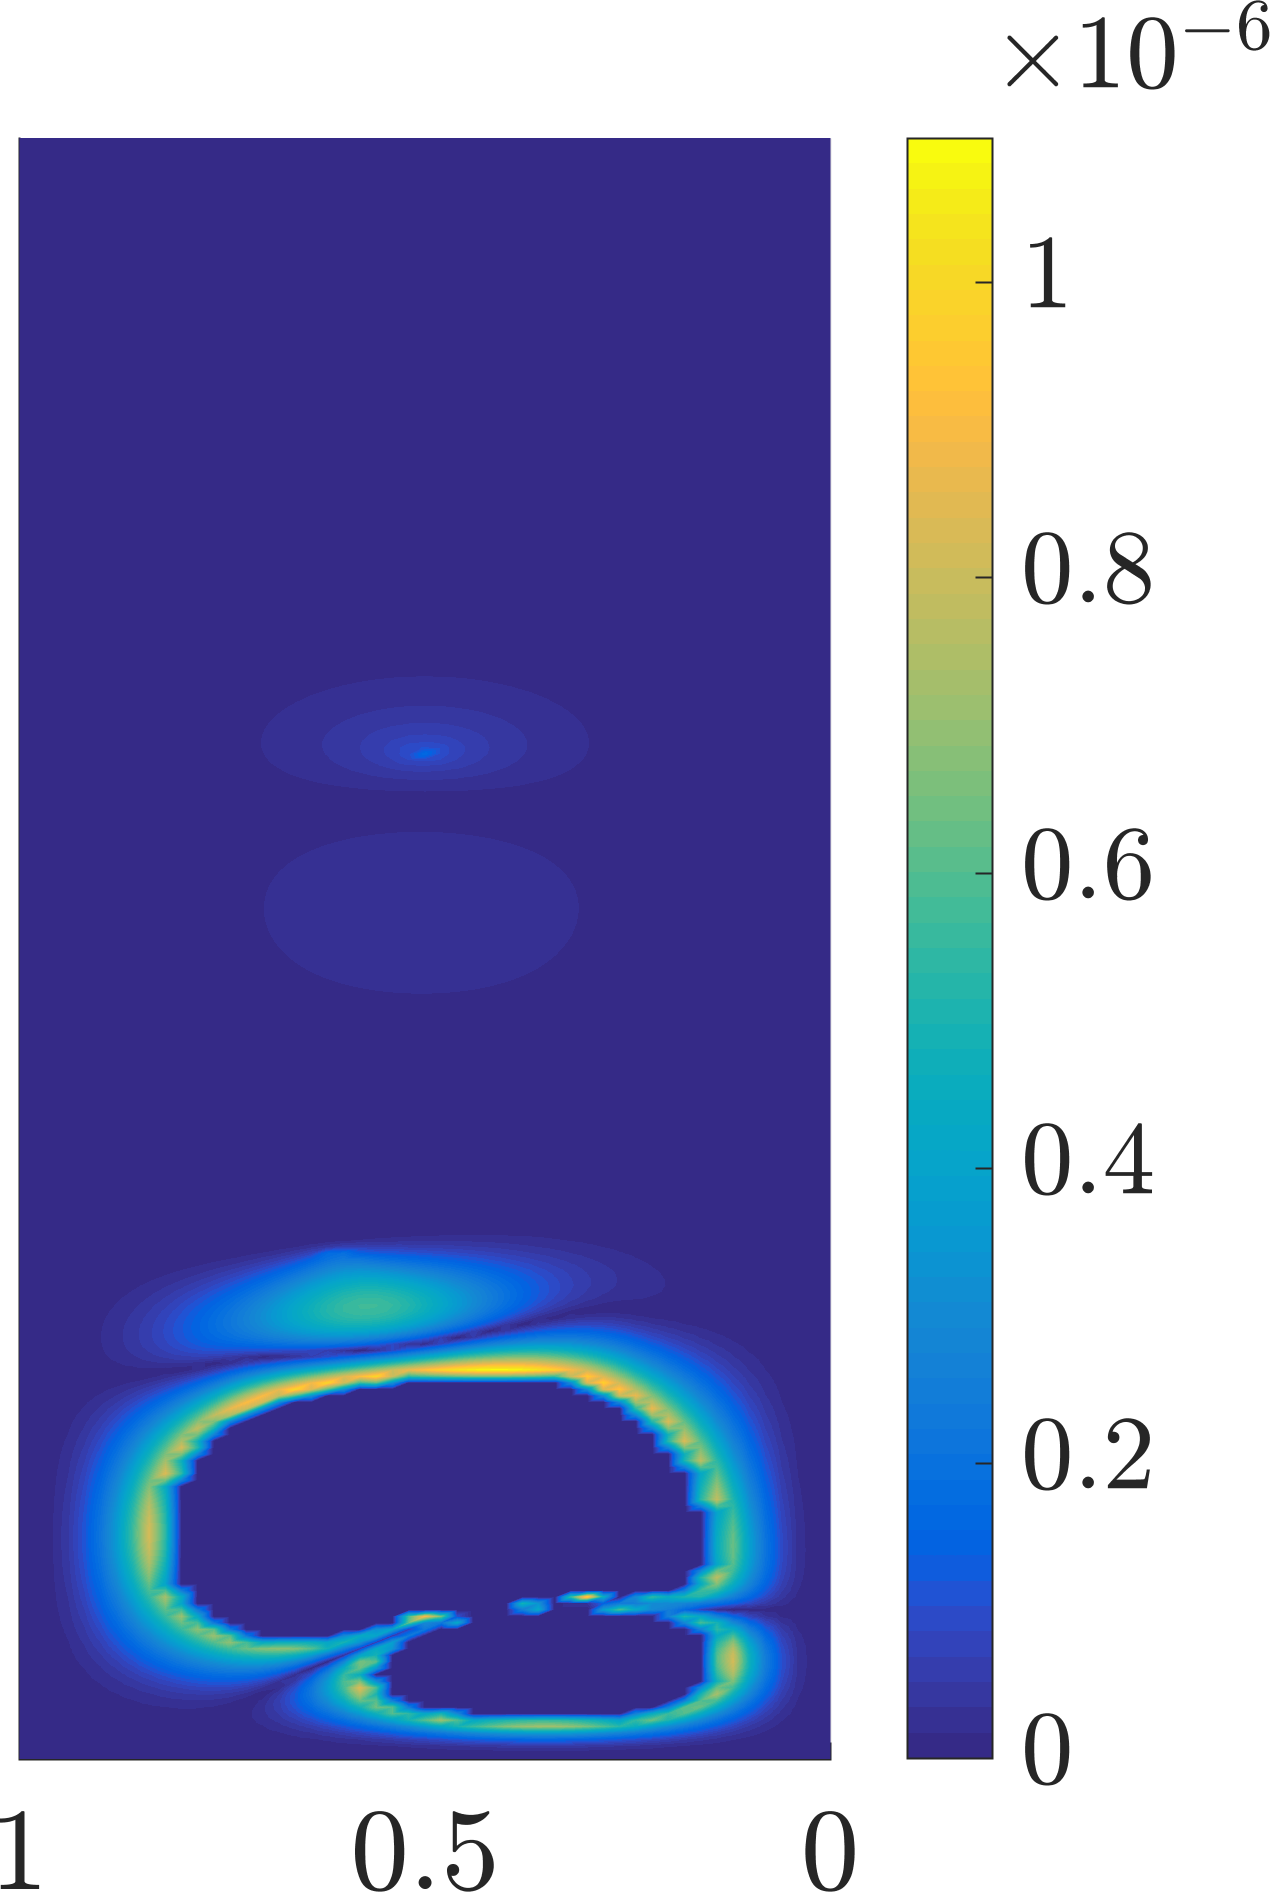
\includegraphics[width=\textwidth]{vs_qoi/qoi7_sens3/err_breakdown_2.png}
    \includegraphics[width=\textwidth]{vs_qoi/qoi3_sens3/err_breakdown_2.png}
    \caption{MF$_2$ \\ ($\sim10\%$ HF)}
    \label{subfig:obsMFlast}
  \end{subfigure}
  \caption{Compare the error estimate decomposition (\subref{subfig:obsLF}-\subref{subfig:obsMFlast}), given the same observations (teal points in (\subref{subfig:obsSetup})) and varying QoI region (purple box in (\subref{subfig:obsSetup})).}
  \label{fig:qoiStudy}
\end{figure}

The error decomposition for three increasing, nested sets of observations and the same QoI region $\Omega_I$ is shown in Figure \ref{fig:dataStudy}. Again, the bottom row gives the baseline case presented in Section~\ref{sec:cdvcdrBaseRef}, although here the basis functions with the largest $5\%$ of the error are chosen, so the proportion of additional refined elements in each iteration is slightly larger. Refinement appears to be consistently most important around the data point closest to $x_1=0$ and the QoI region. However, as more data points are added, it becomes no longer necessarily true that refinement becomes less important around data points as their distance from the QoI region increases. The data points also interact with each other in that placing data points in regions of previously relatively uniform error contribution tends to result in a new error decomposition that is positive or negative around the data points, with valleys of zero magnitude in between.

\begin{figure}
\captionsetup[subfigure]{justification=centering}
\centering
  \begin{subfigure}[t]{0.20\textwidth}
  \centering
    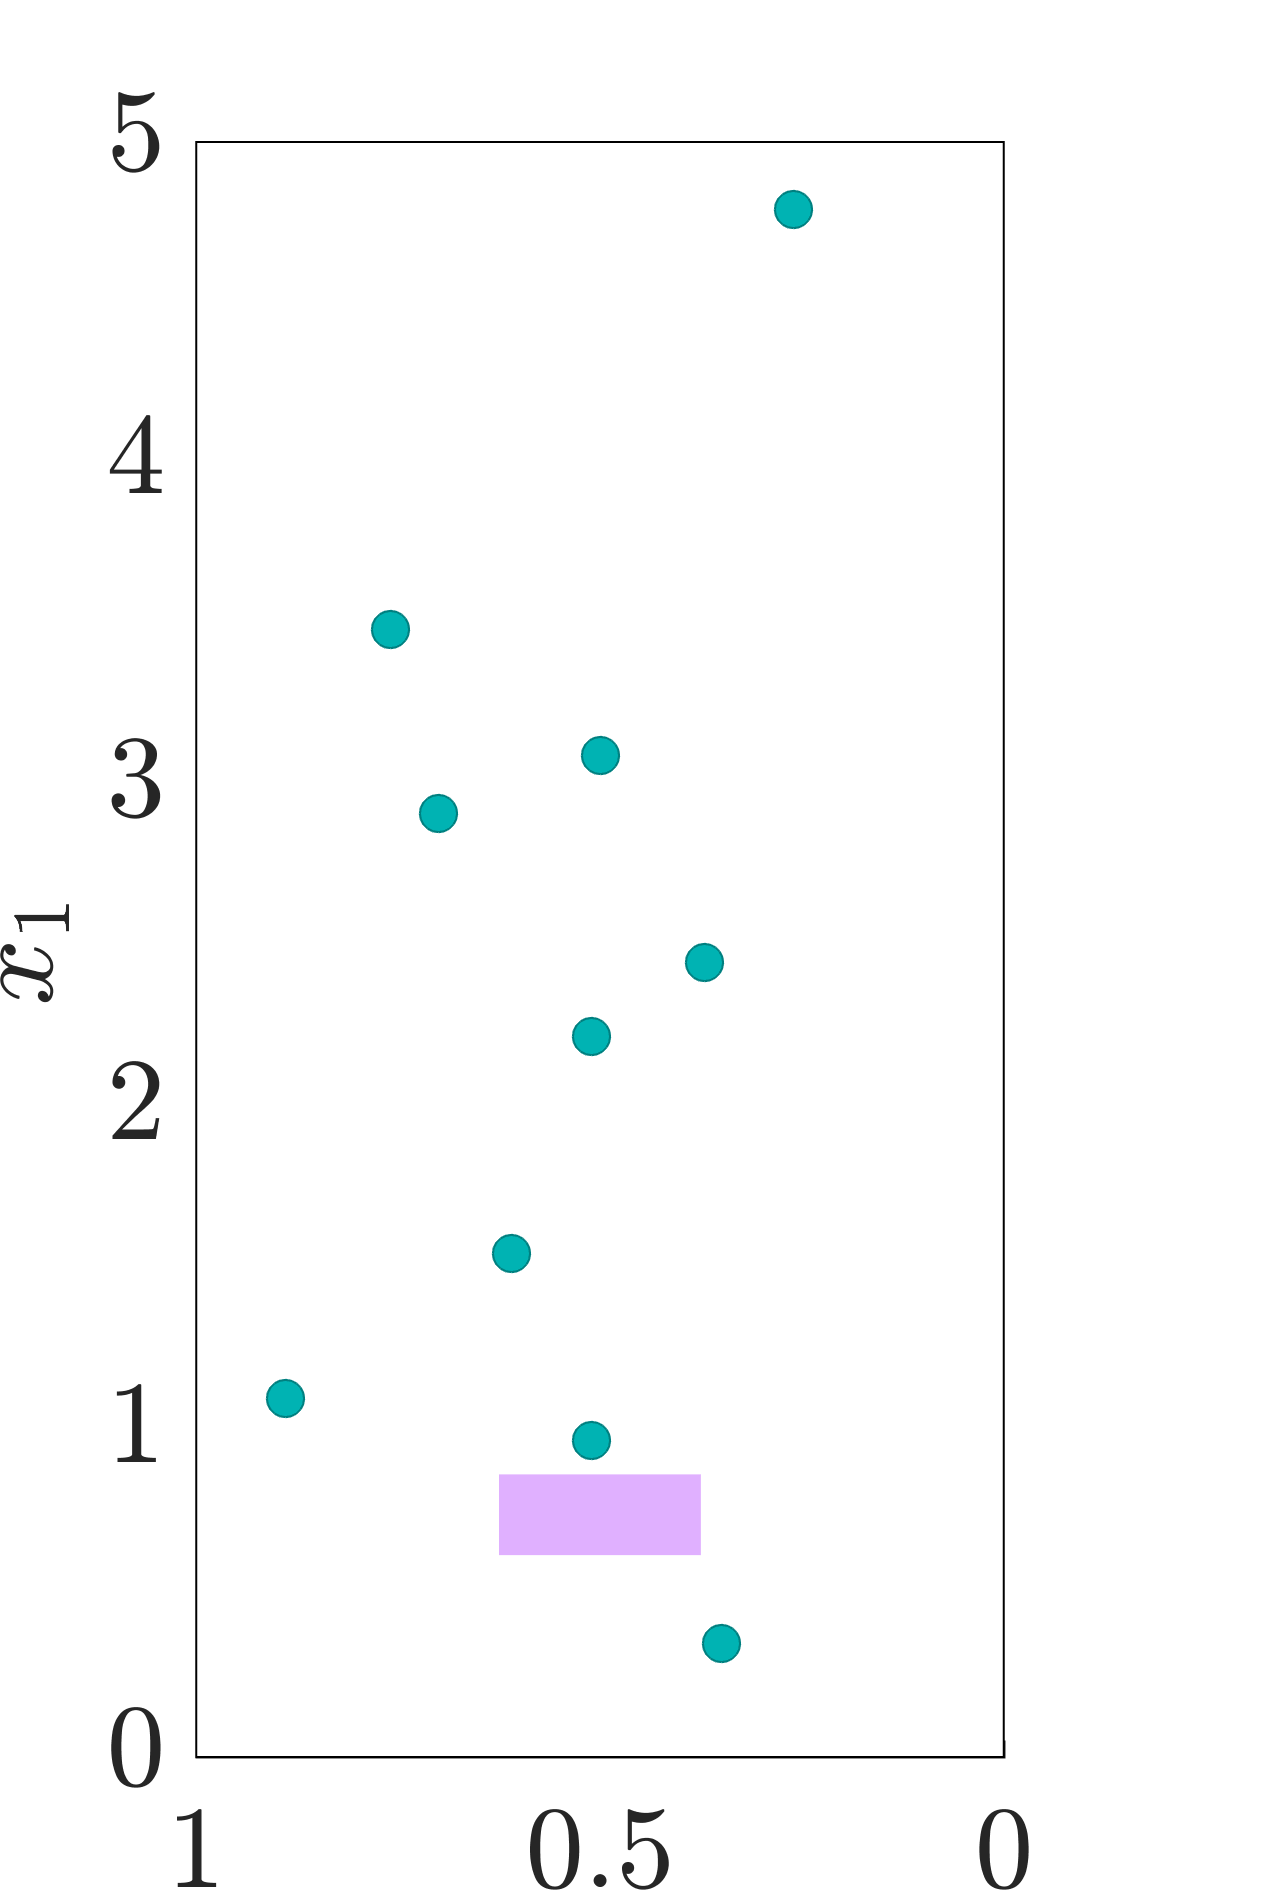
\includegraphics[width=\textwidth]{vs_data/qoi3_sens10/setup_3_10.png}
    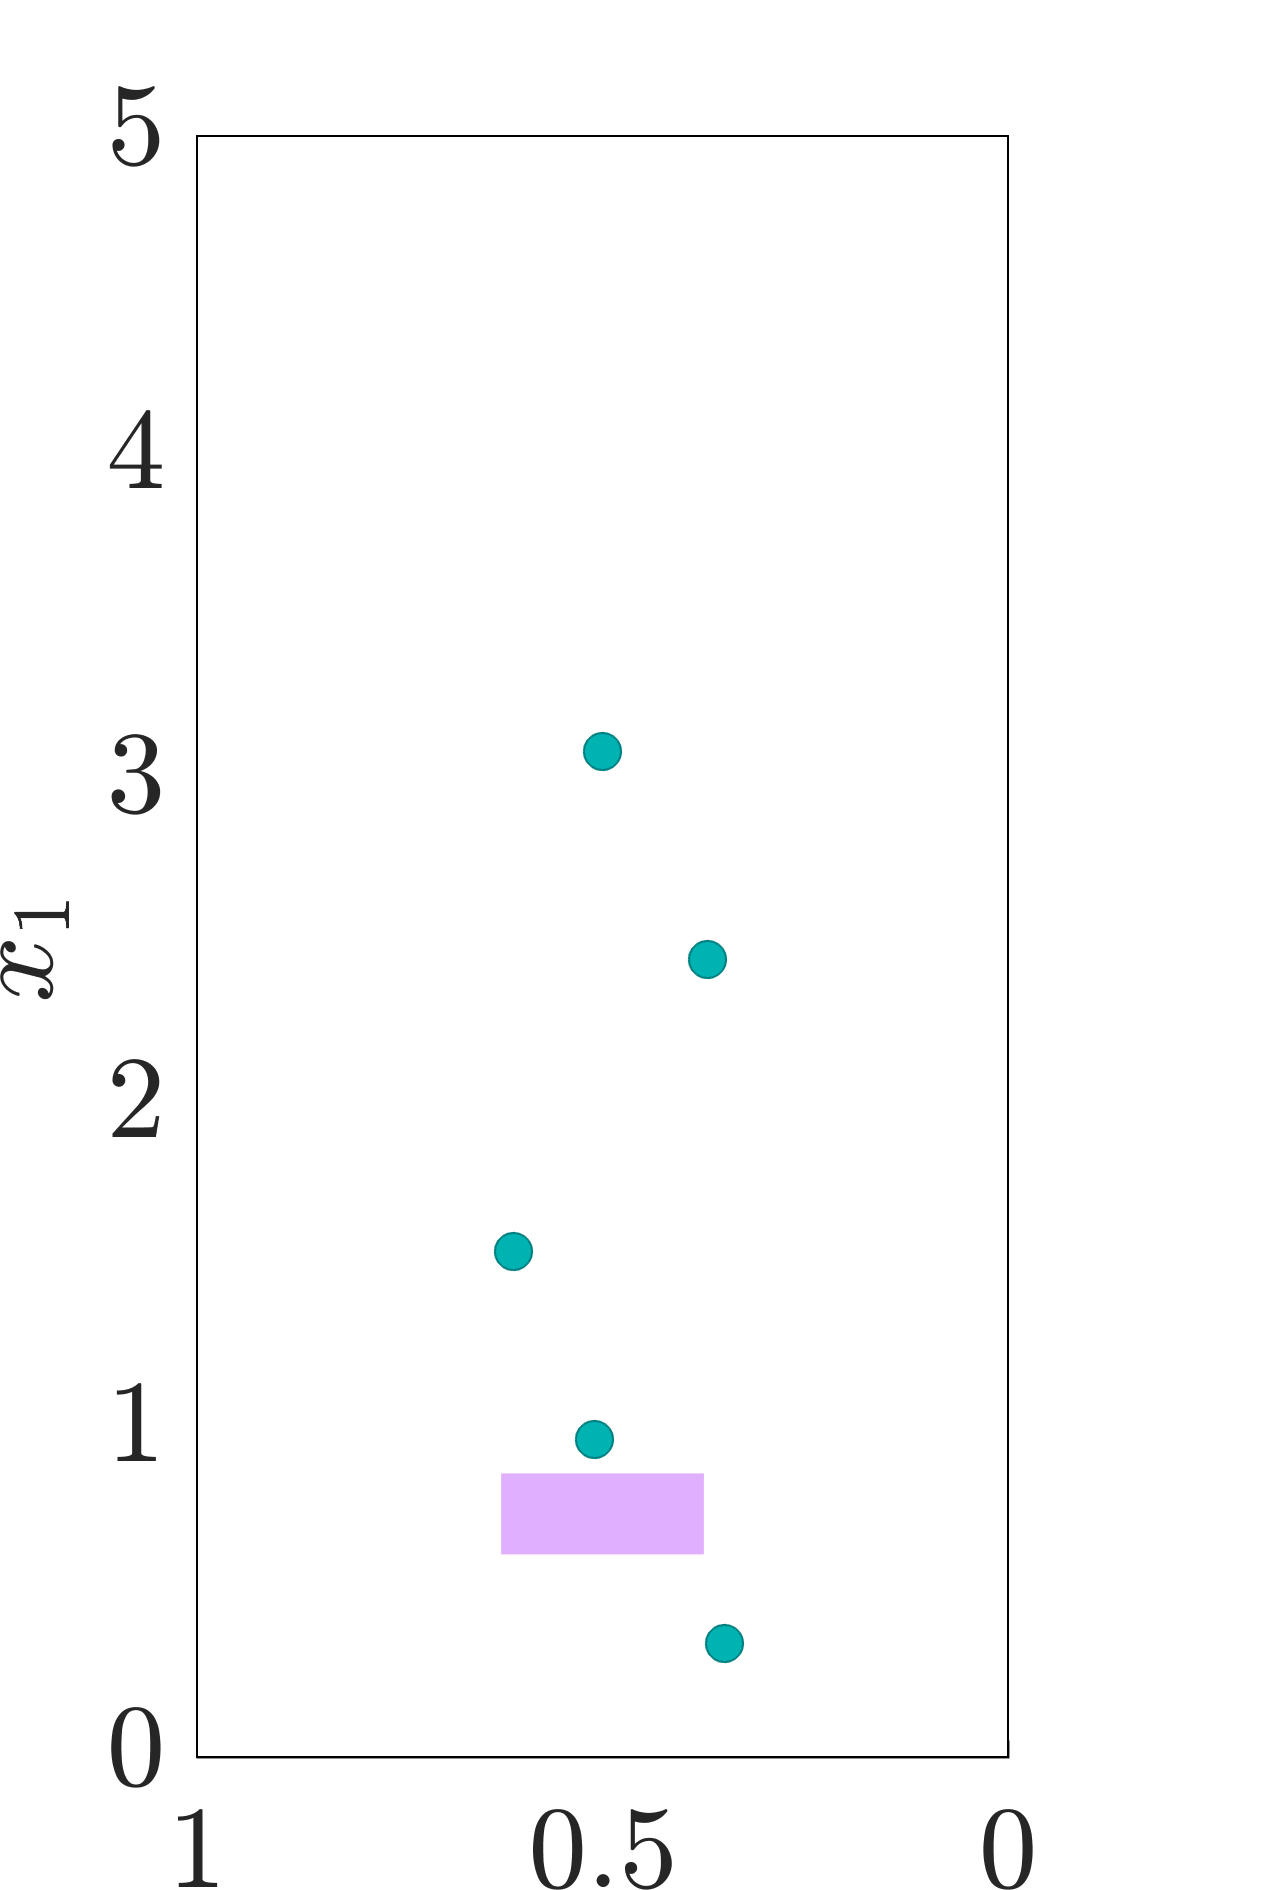
\includegraphics[width=\textwidth]{vs_data/qoi3_sens5/setup_3_5.png}
    \includegraphics[width=\textwidth]{vs_data/qoi3_sens3/setup_3_3.png}
    \caption{Locations of observations and QoI region $\Omega_I$}
    \label{subfig:obsSetup2}
  \end{subfigure}
  \begin{subfigure}[t]{0.20\textwidth}
  \centering
    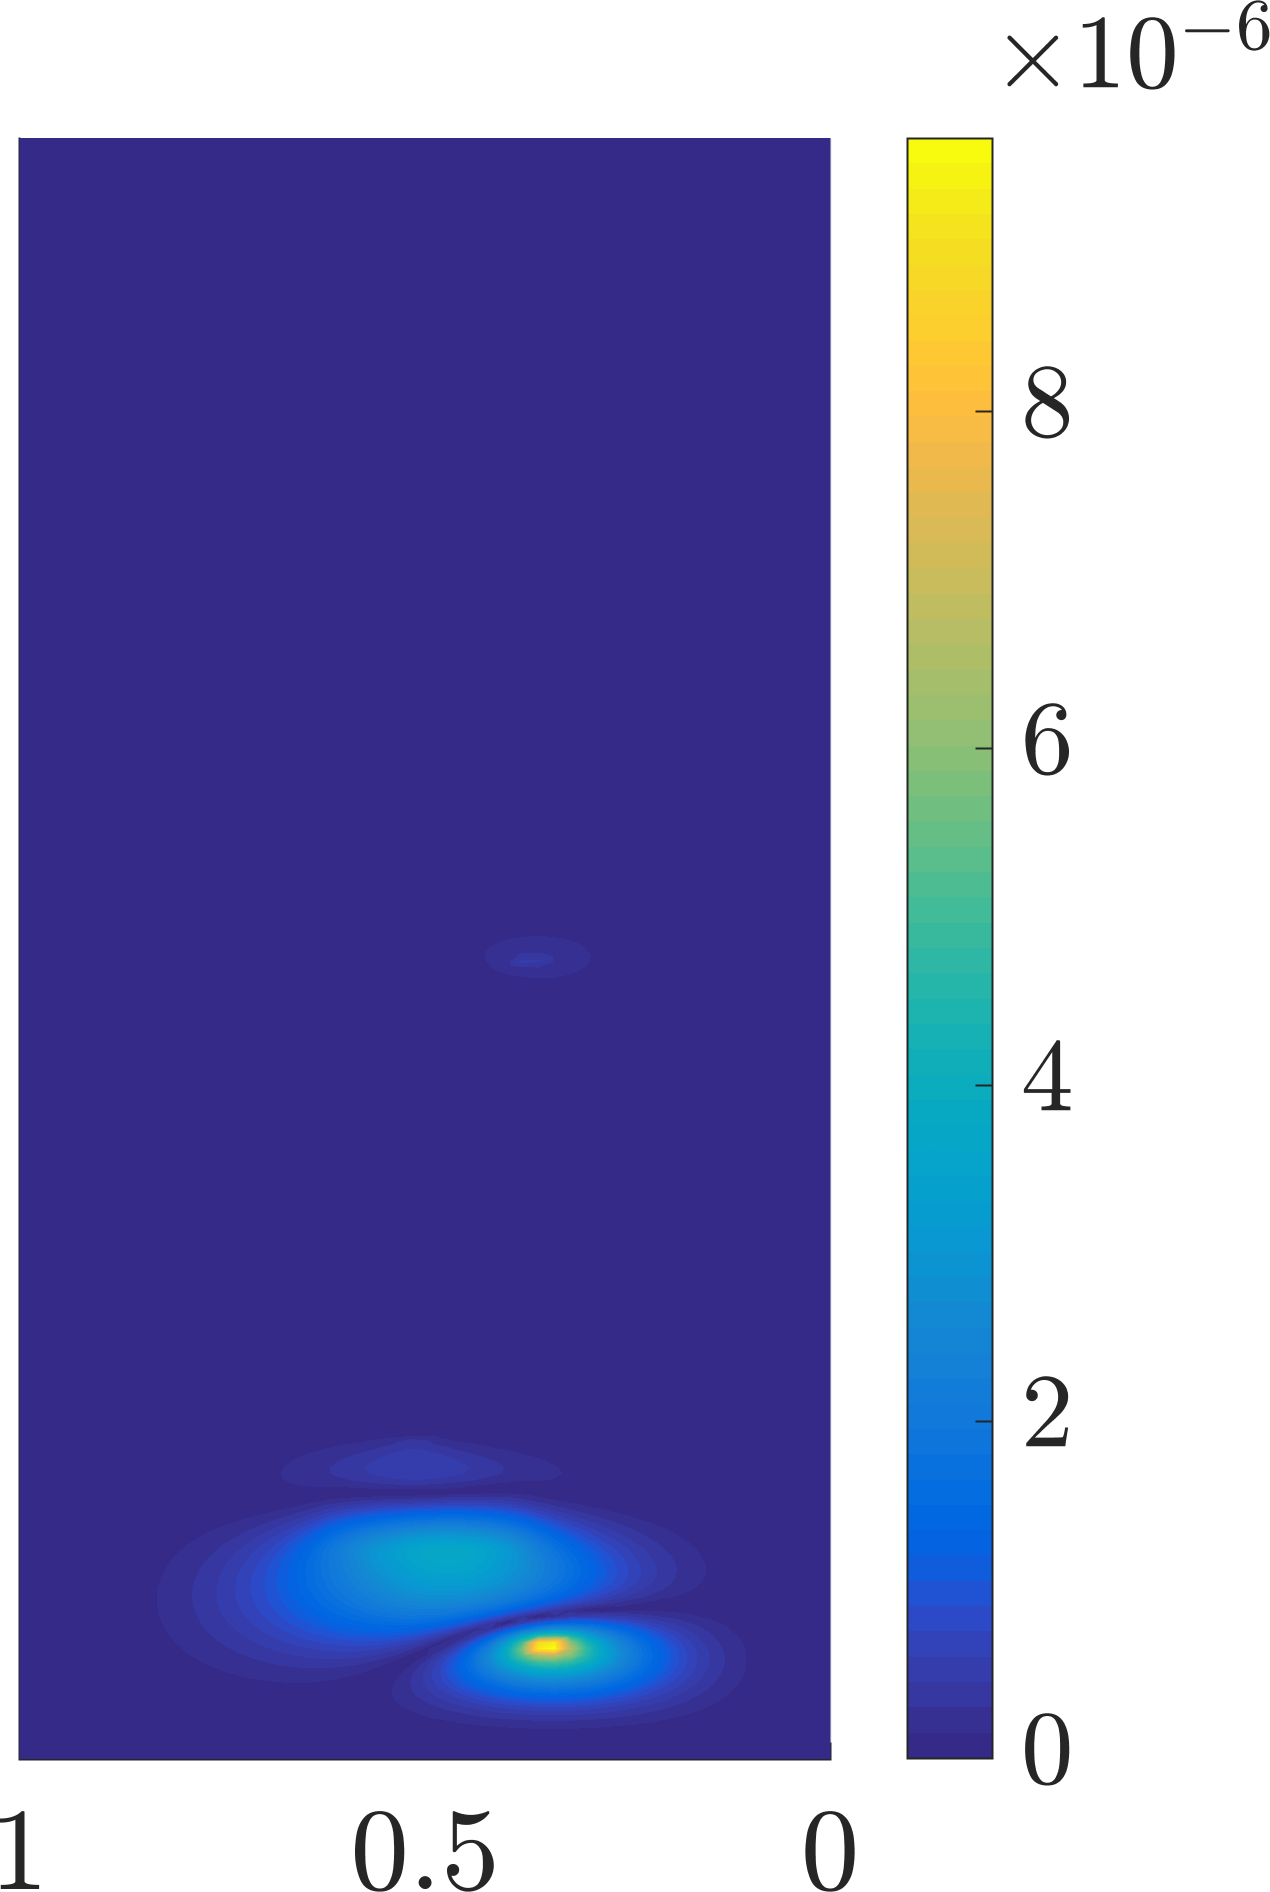
\includegraphics[width=\textwidth]{vs_data/qoi3_sens10/err_breakdown_0.png}
    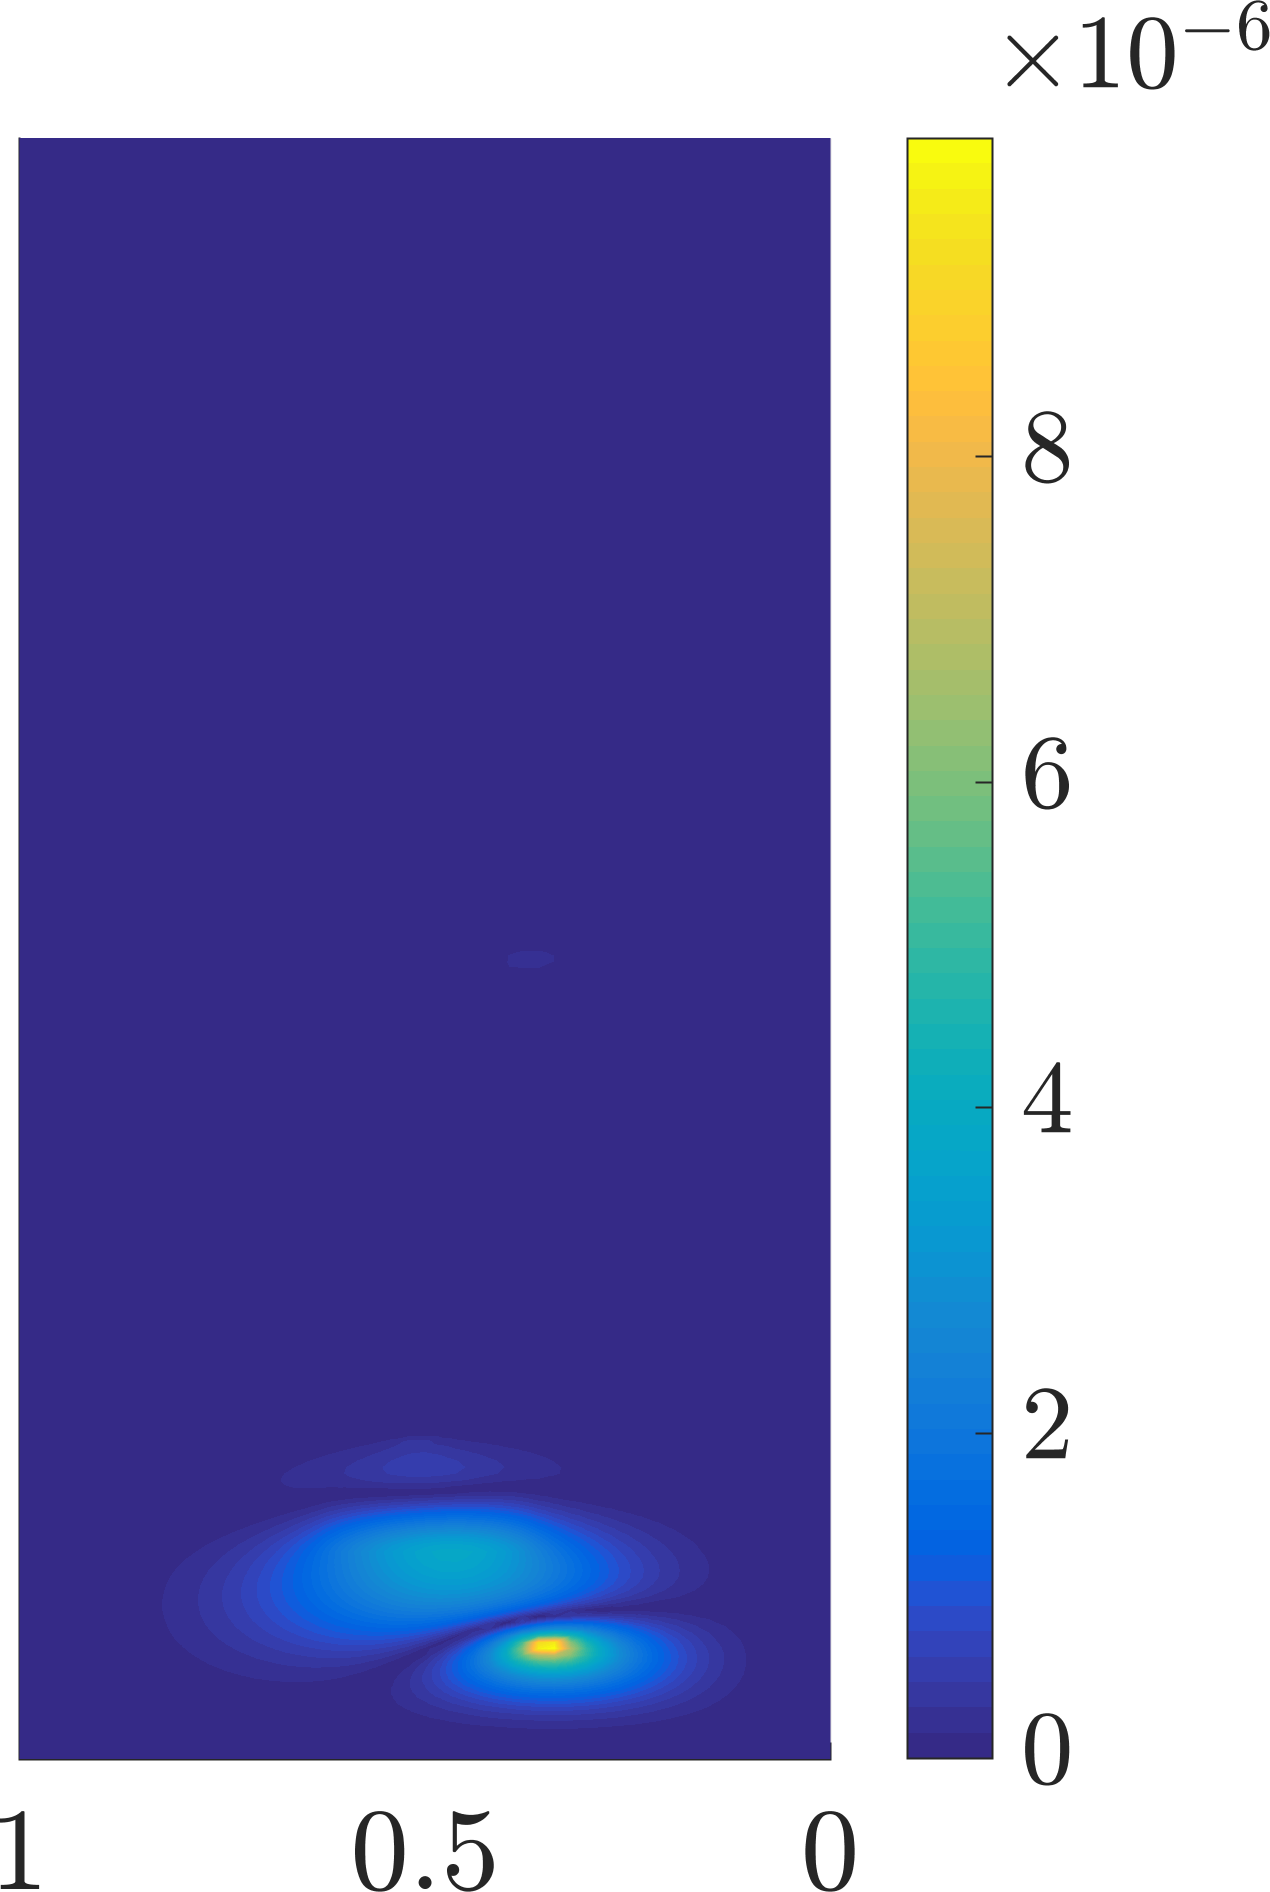
\includegraphics[width=\textwidth]{vs_data/qoi3_sens5/err_breakdown_0.png}
    \includegraphics[width=\textwidth]{vs_data/qoi3_sens3/err_breakdown_0.png}
    \caption{MF$_0$ \\ ($0\%$ HF)}
    \label{subfig:obsLF2}
  \end{subfigure}
  \begin{subfigure}[t]{0.20\textwidth}
  \centering
    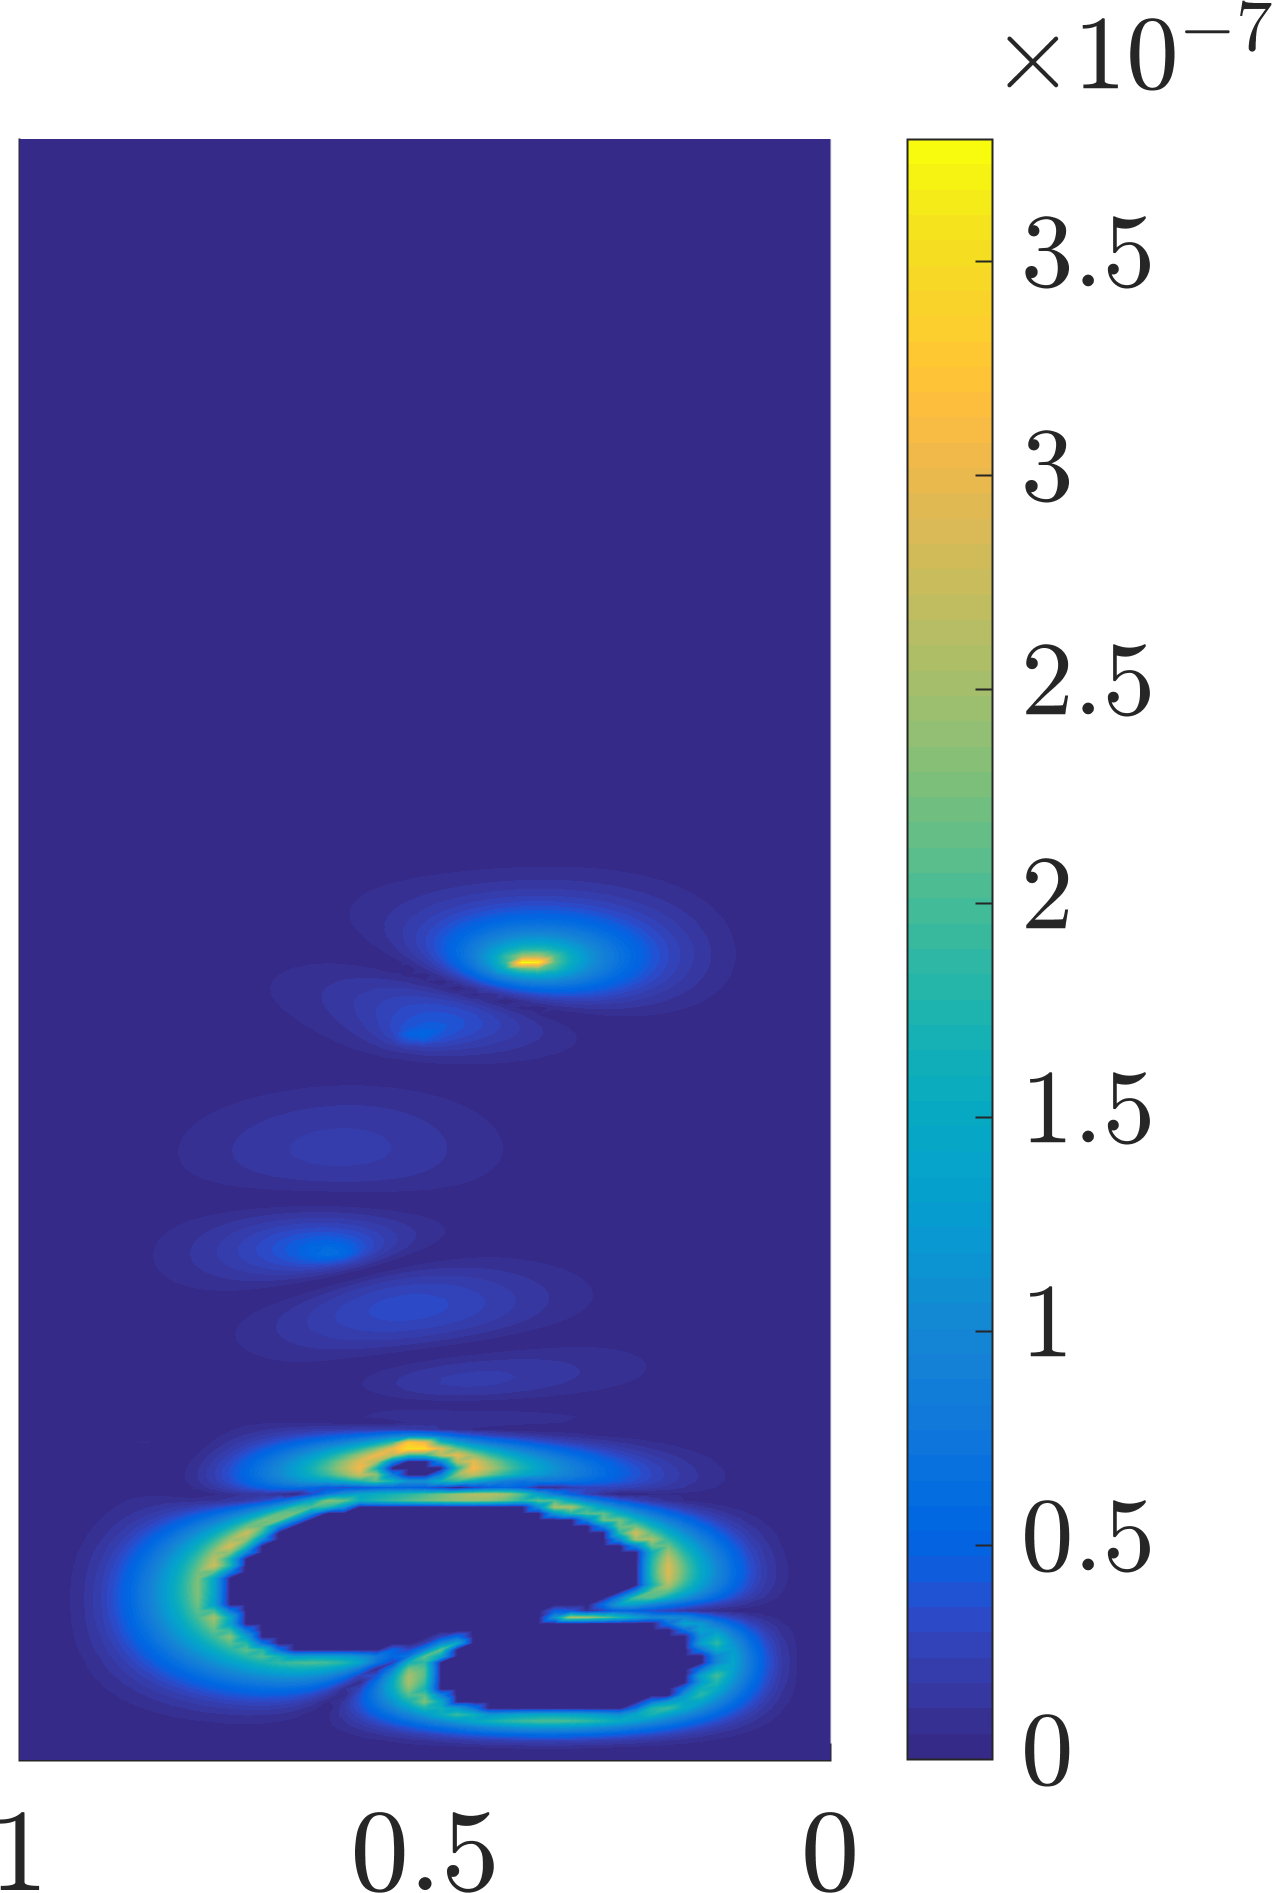
\includegraphics[width=\textwidth]{vs_data/qoi3_sens10/err_breakdown_1.png}
    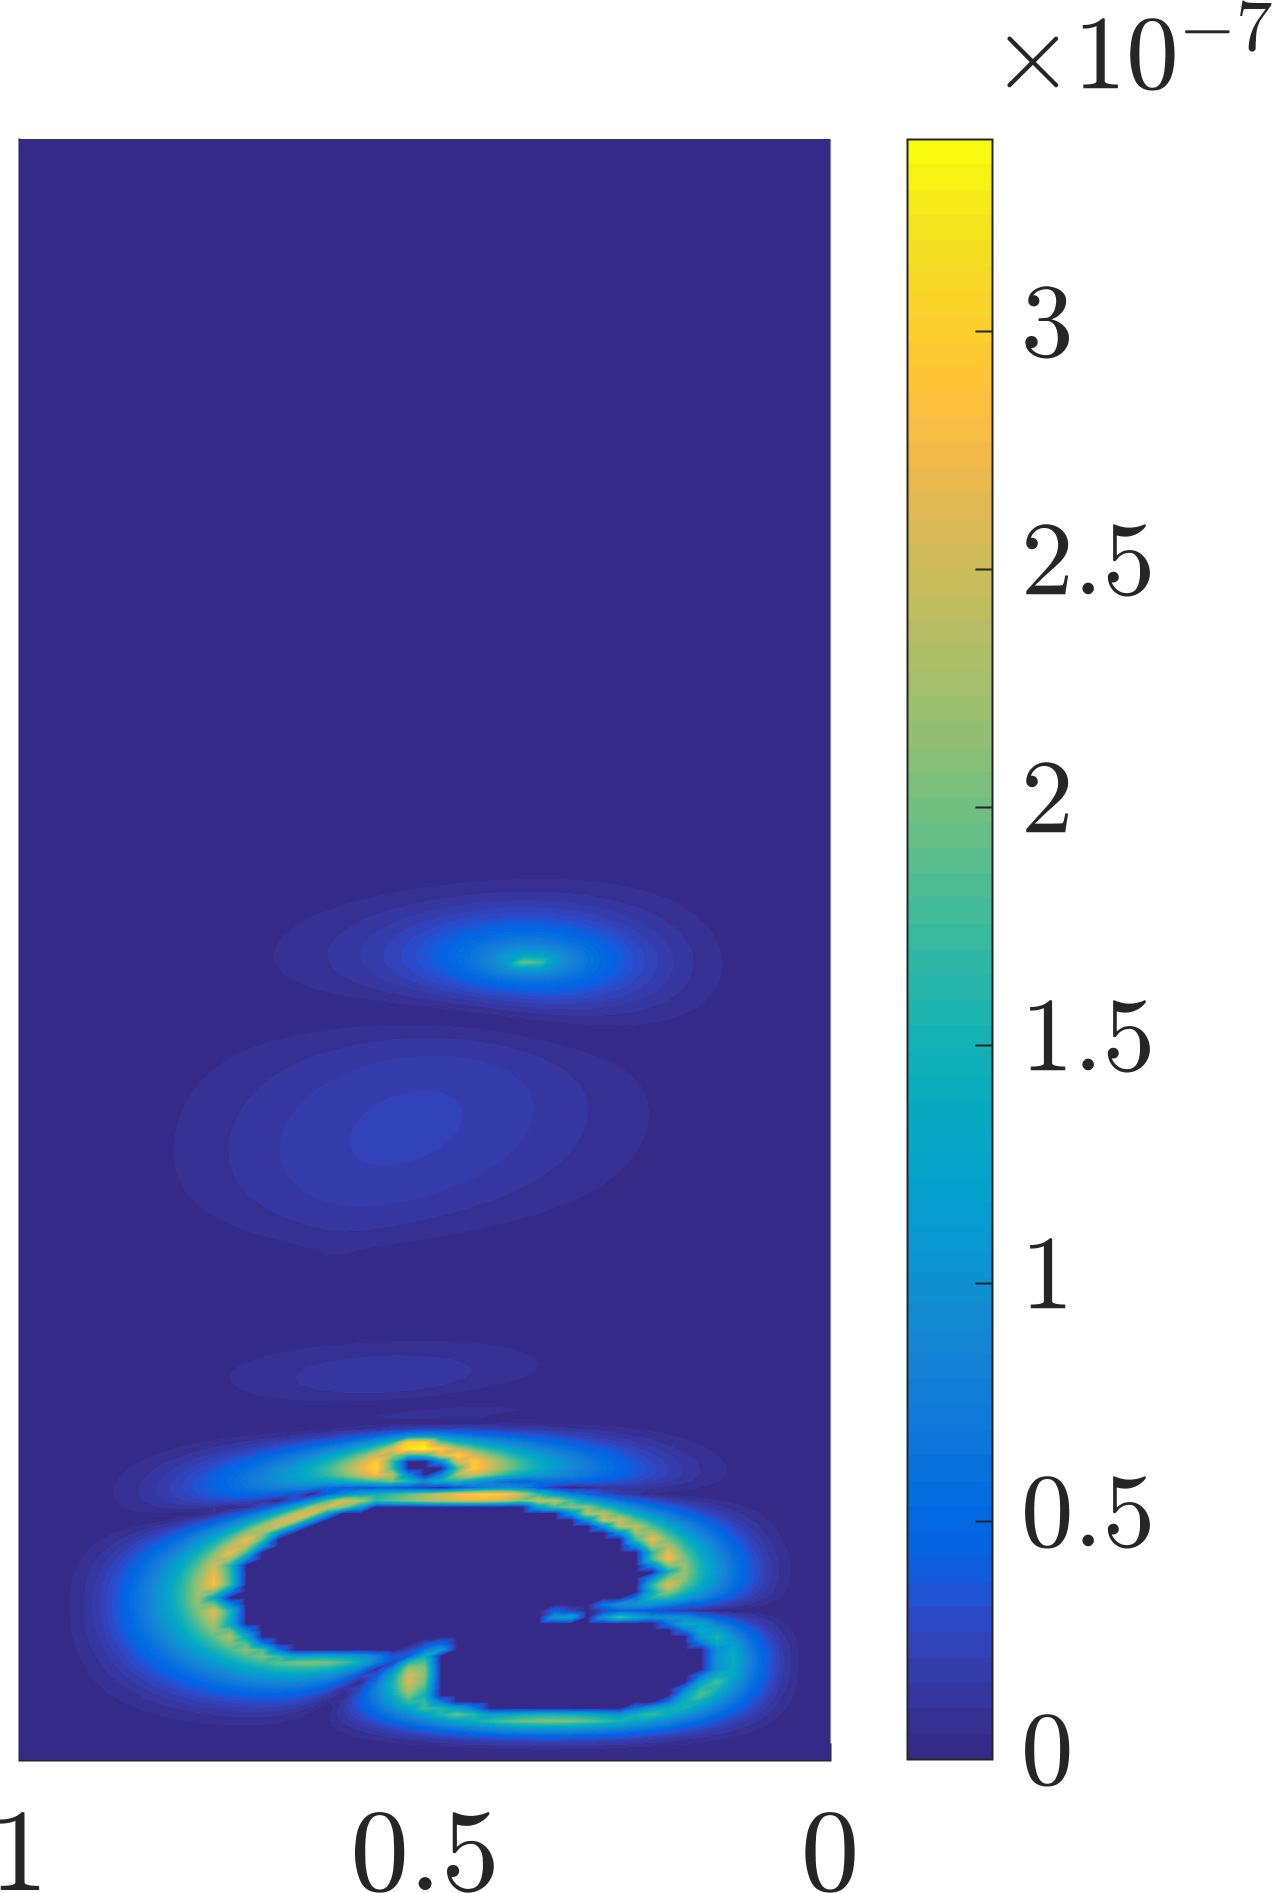
\includegraphics[width=\textwidth]{vs_data/qoi3_sens5/err_breakdown_1.png}
    \includegraphics[width=\textwidth]{vs_data/qoi3_sens3/err_breakdown_1.png}
    \caption{MF$_1$ \\ ($\sim5\%$ HF)}
  \end{subfigure}
  \begin{subfigure}[t]{0.20\textwidth}
  \centering
    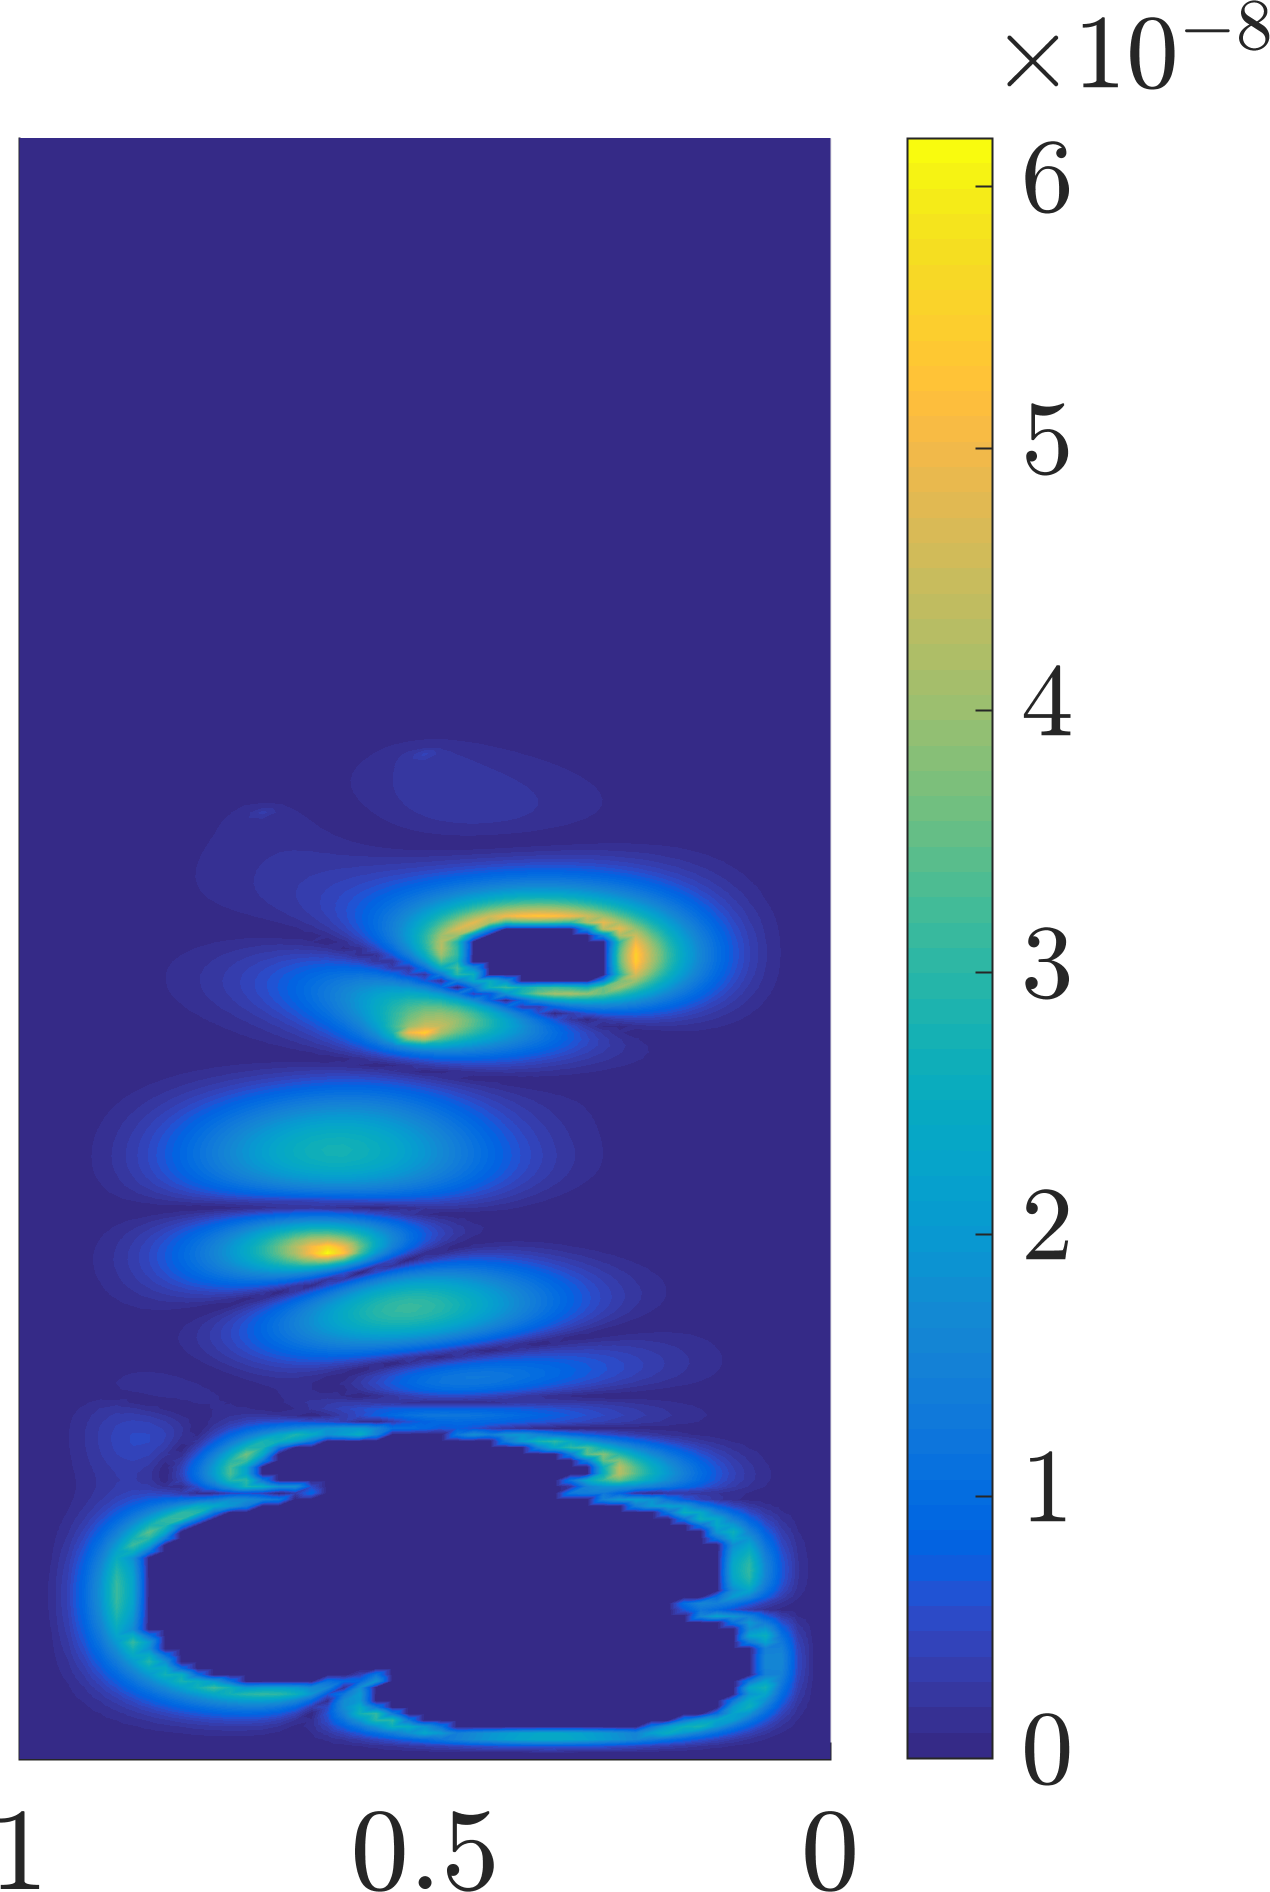
\includegraphics[width=\textwidth]{vs_data/qoi3_sens10/err_breakdown_2.png}
    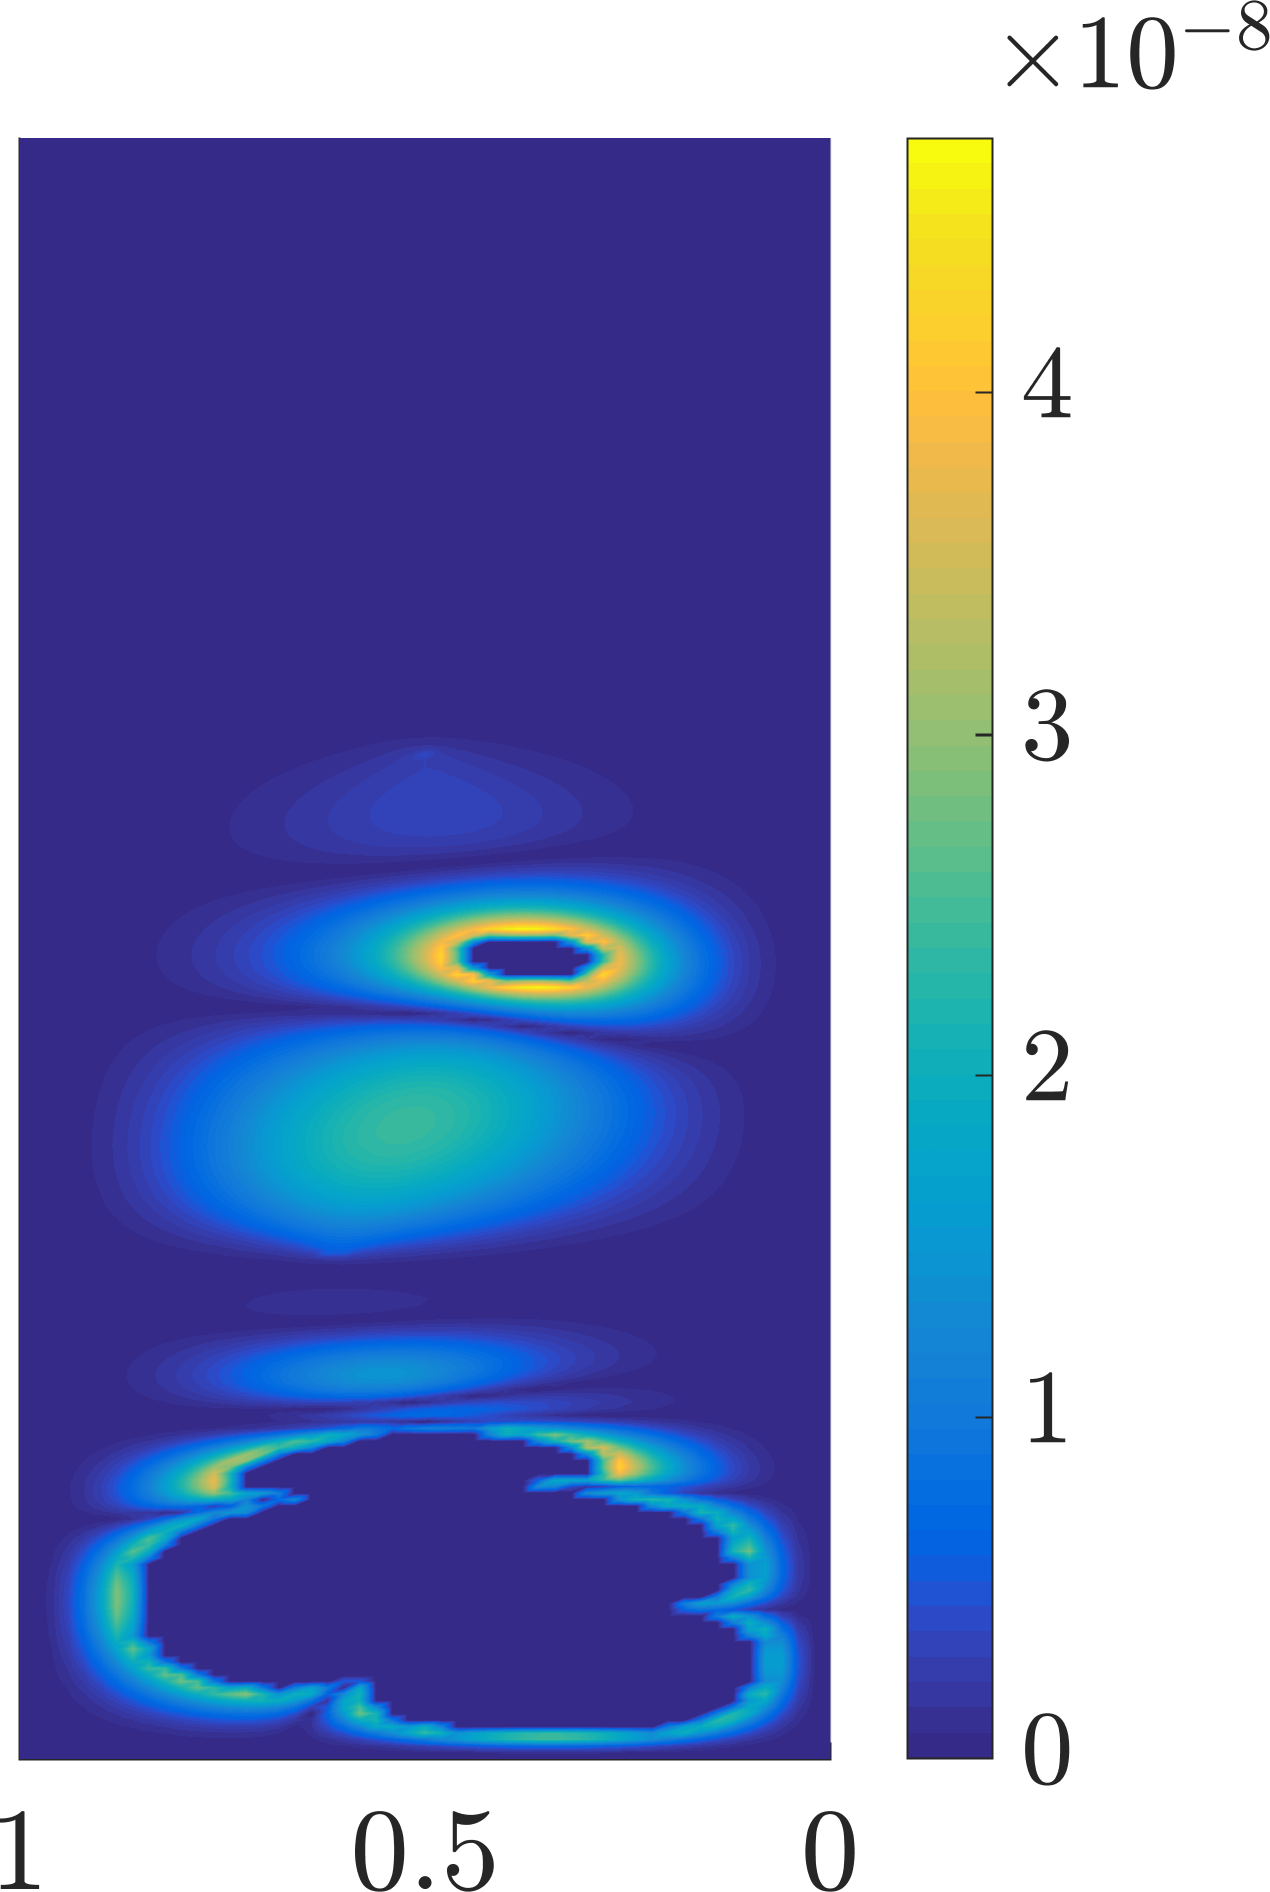
\includegraphics[width=\textwidth]{vs_data/qoi3_sens5/err_breakdown_2.png}
    \includegraphics[width=\textwidth]{vs_data/qoi3_sens3/err_breakdown_2.png}
    \caption{MF$_2$ \\ ($\sim10\%$ HF)}
    \label{subfig:obsMFlast2}
  \end{subfigure}
  \caption{Compare the error estimate decomposition (\subref{subfig:obsLF2}-\subref{subfig:obsMFlast2}), given the same QoI region (purple box in (\subref{subfig:obsSetup2})) and varying observations (teal points in (\subref{subfig:obsSetup2})).}
  \label{fig:dataStudy}
\end{figure}

%
\subsection{Constant vs Field Parameters}
%
\subsubsection{Problem Setup}
%
\subsubsection{Results}
%
%bigger steps in 3D problem because qoi region bigger?
\subsection{Convection-Diffusion(-Highly Nonlinear Reaction)}
%
\subsubsection{Results}
%
We consider the convection-diffusion-reaction term described in Section \ref{sec:cdvcdr}, with a reaction term $k_r=-616$ in the high-fidelity model. This reaction term is large enough that the Newton solver will not converge with a zero initial guess. We first solve the inverse problem with the low-fidelity model ($k_r=0$), and then use a simple continuation approach, using the solution at one value of $k_r$ as the initial guess for the next.\footnote{not arclength continuation, which is more difficult to implement, though libMesh appears to have a class for such continuation, which we can use if this seems like a viable direction} We increase the reaction term in increments of $\Delta k_r=100$, and halve the increment each time the step is too large (Newton solver does not converge at the next $k_r$ value). From $k_r=0$ to $k_r=-616$, this results in 9 continuation steps being taken.
%
\subsubsection{Computational Complexity}
%
We compare the complexity of Algorithm~\ref{alg:refSeries} and the continuation method for the high fidelity problem, in the context of the analysis developed in section~\ref{sect:alg_complexity}. For the high fidelity problem, with  with 9 continuation steps, we have $\sum\limits_{i=1}^{C} K_i=30$. 
 
With Gaussian elimination chosen as the linear solver, this gives us $T < 3$, i.e.\ a budget of 2 adaptive steps. Using Algorithm~\ref{alg:refSeries} with 2 refinement steps, and only $10\%$ of the domain refined to use the high-fidelity model, the estimated relative error is $<1\%$. Indeed, the ratio $\frac{C_{MF}}{C_{HF}}$ was $\frac{24}{30}$, indicating about $20\%$ reduction in computational cost, with the worst case linear solver used. 

In other words, on using Algorithm~\ref{alg:refSeries} for a highly nonlinear problem, even with the worst case linear solver, one can get to $<1\%$ error in the QoI, with a $20\%$ reduction in computational cost, while avoiding any need for continuation to handle nonlinearities. 

\section{Conclusion}


\appendix
%\chapter{Notation} \label{appendix}

For quick reference, the following table summarizes notation used throughout this thesis 
(in alphabetical order).

\begin{table}[!ht]
\caption{Summary of Notation}
\begin{center}
\begin{tabular}{c|l}
\textbf{Symbol} & \textbf{Meaning} \\
\hline \hline
$q$  &   Model parameters \\
$u$  &   Model state\\
\end{tabular}
\end{center}
\end{table}

%% This defines the bibliography file (main.bib) and the bibliography style.
%% If you want to create a bibliography file by hand, change the contents of
%% this file to a `thebibliography' environment.  For more information 
%% see section 4.3 of the LaTeX manual.
\begin{singlespace}
\addcontentsline{toc}{chapter}{\hspace{3ex}Bibliography}
\bibliography{masterBib}
\bibliographystyle{plain}
\end{singlespace}

\end{document}
